\subsection{Respuesta en frecuencia del circuito}

\subsubsection{An\'alisis te\'orico} %%%%%%%

\subsubsection*{Configuraci\'on inversora}
Se calcula de forma te\'orica la ganancia del circuito \ref{c1}, 
considerando al amplificador operacional como ideal, es decir, 
con impedancia de entrada infinita e impedancia de salida nula. Se parte de las siguientes ecuaciones:
\begin{equation}
	\begin{cases}
		V_{out} = A_{vol}\cdot(V^+ - V^-) = -A_{vol} V^- \cdot \\
		V_{in} - R_1 \cdot I_1 = V^- \\
		V_{out} - R_2 \cdot I_2 = V^-\\ 
		I_3 = I_1 + I_2
	\end{cases}
	\label{ecsbase}
\end{equation}

Operando matem\'aticamente se obtiene la siguiente expresi\'on:

\begin{equation}
	\frac{V_{out}}{V_{in}} = - \frac{R_2/R_1}{1 + \frac{R_2/R_1}{A_{vol}} + \frac{R_2/R_3}{A_{vol}}}
	\label{c1vovi}
\end{equation}

\subsubsection*{Considerando $A_{vol} $finito}
 
En la tabla \ref{avolf} se puede ver el valor correspondiente a cada caso, obtenido al considerar 
$A_{vol} = A_{V0} = 100000$, cuyo valor fue sacado de la hoja de datos del LM324.

\begin{table}[h!]
	\centering
	\begin{tabular}{c c c}%
		\bfseries  & $V_{out}/V_{in}$ & $|V_{out}/V_{in}| (dB)$ \\ \hline
		caso 1 & $-9,998$ & $19,998$\\
		caso 2 & $ -1,00$ & $0,000$ \\
		caso 3 & $ -0,100$ & $-20,000$\\
		\hline
	\end{tabular}
	\caption{$V_{out}/V_{in}$ del circuito inversor considerando $A_{vol}$ finito.}
	\label{avolf}
\end{table}

En la tabla \ref{avolf} se observa que para la configuraci\'on del circuito \ref{c1} hay una ganancia de casi $20dB$ para el caso 1 de la distribuci\'on de resistencias, mientras que para el caso 2 no hay ganancia ni atenuaci\'on y para el caso 3 hay atenuaci\'on de $20dB$.  El resultado obtenido
no var\'ia con la frecuencia ya que el circuito es resistivo y se consider\'o,
para lo calculado reci\'en, que $A_{vol}$ no var\'ia con la frecuencia. Estos resultados
fueron obtenidos para cont\'inua ya que es el caso en el que $A_{vol}=A_{V0}$,
dado que: $A_{vol} = \frac{A_{V0}}{1+s/\omega_p} $ y cuando la frecuencia es cero,
este valor tiende a $A_{V0}$. Otra cosa que se observa en la tabla, son los signos de las relaciones de tensiones de salida respecto a las de entrada. El hecho de que los valores hayan dado negativos, corresponde con que se trata de un circuito de configuraci\'on inversora.


Por otro lado, reemplazando en la ecuaci\'on \ref{c1vovi} con los valores
 correspondientes de resistencias para cada uno de los tres casos
  (indicados en la tabla \ref{casos}) y considerando
   $A_{vol}(\omega)$ (con $s = j\omega$), se obtienen las siguientes expresiones:

Caso1:
\begin{equation}
	\frac{V_{out}}{V_{in}} = - \frac{7\cdot10^{12}}{2088,9 \cdot 10^3 s + 7 \cdot 10^{11}}
	\label{c1c1vovi}
\end{equation}

caso 2:
\begin{equation}
	\frac{V_{out}}{V_{in}} = - \frac{7 \cdot 10^{11}}{298,4 \cdot 10^{3} s +7 \cdot 10^{11}}
	\label{c1c2vovi}
\end{equation}

caso 3:
\begin{equation}
	\frac{V_{out}}{V_{in}} = - \frac{7 \cdot 10^{12}}{119,366 \cdot 10^{5} s +7 \cdot 10^{13}}
	\label{c1c3vovi}
\end{equation}

A continuaci\'on en los gr\'aficos \ref{c1voviTeoMod} y \ref{c1voviTeoPh} se observa c\'omo var\'ia la ganancia del circuito para los tres casos en funci\'on de la frecuencia.

\begin{figure}[H] %!ht
	\centering
	%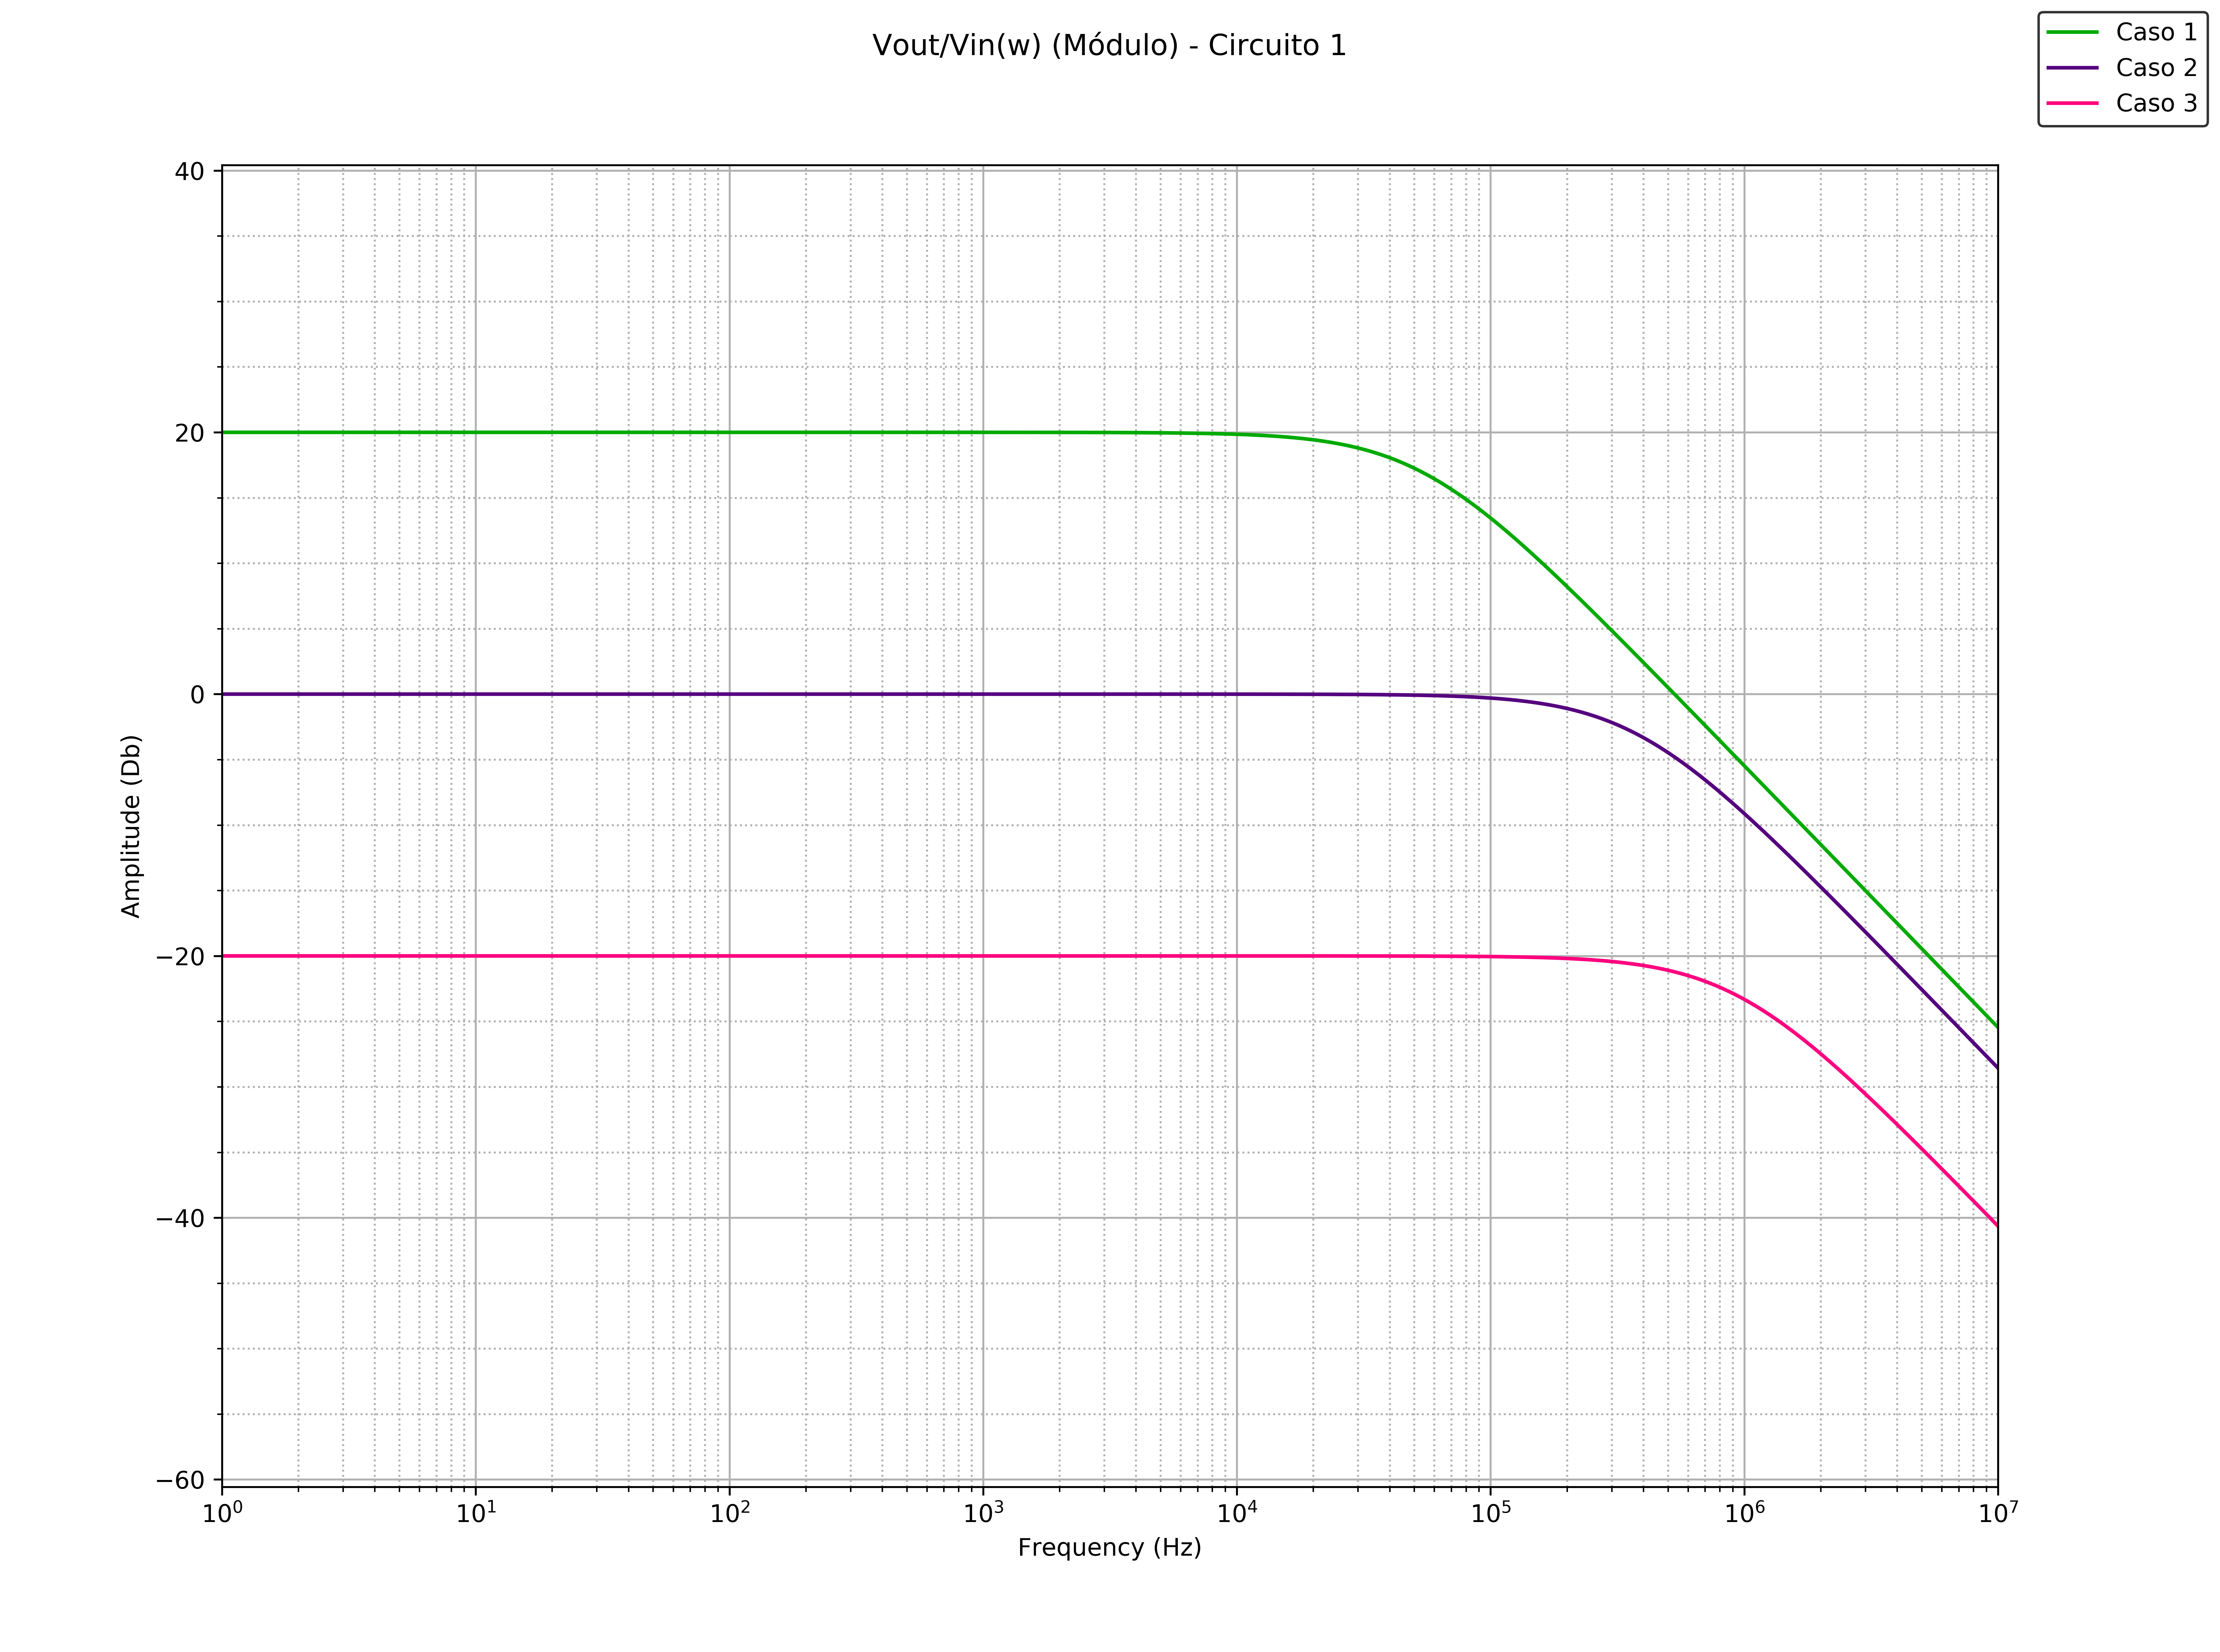
\includegraphics[scale=0.45]{../EJ1/00GRAFICOS/teoricos/circ1voviw.png}
	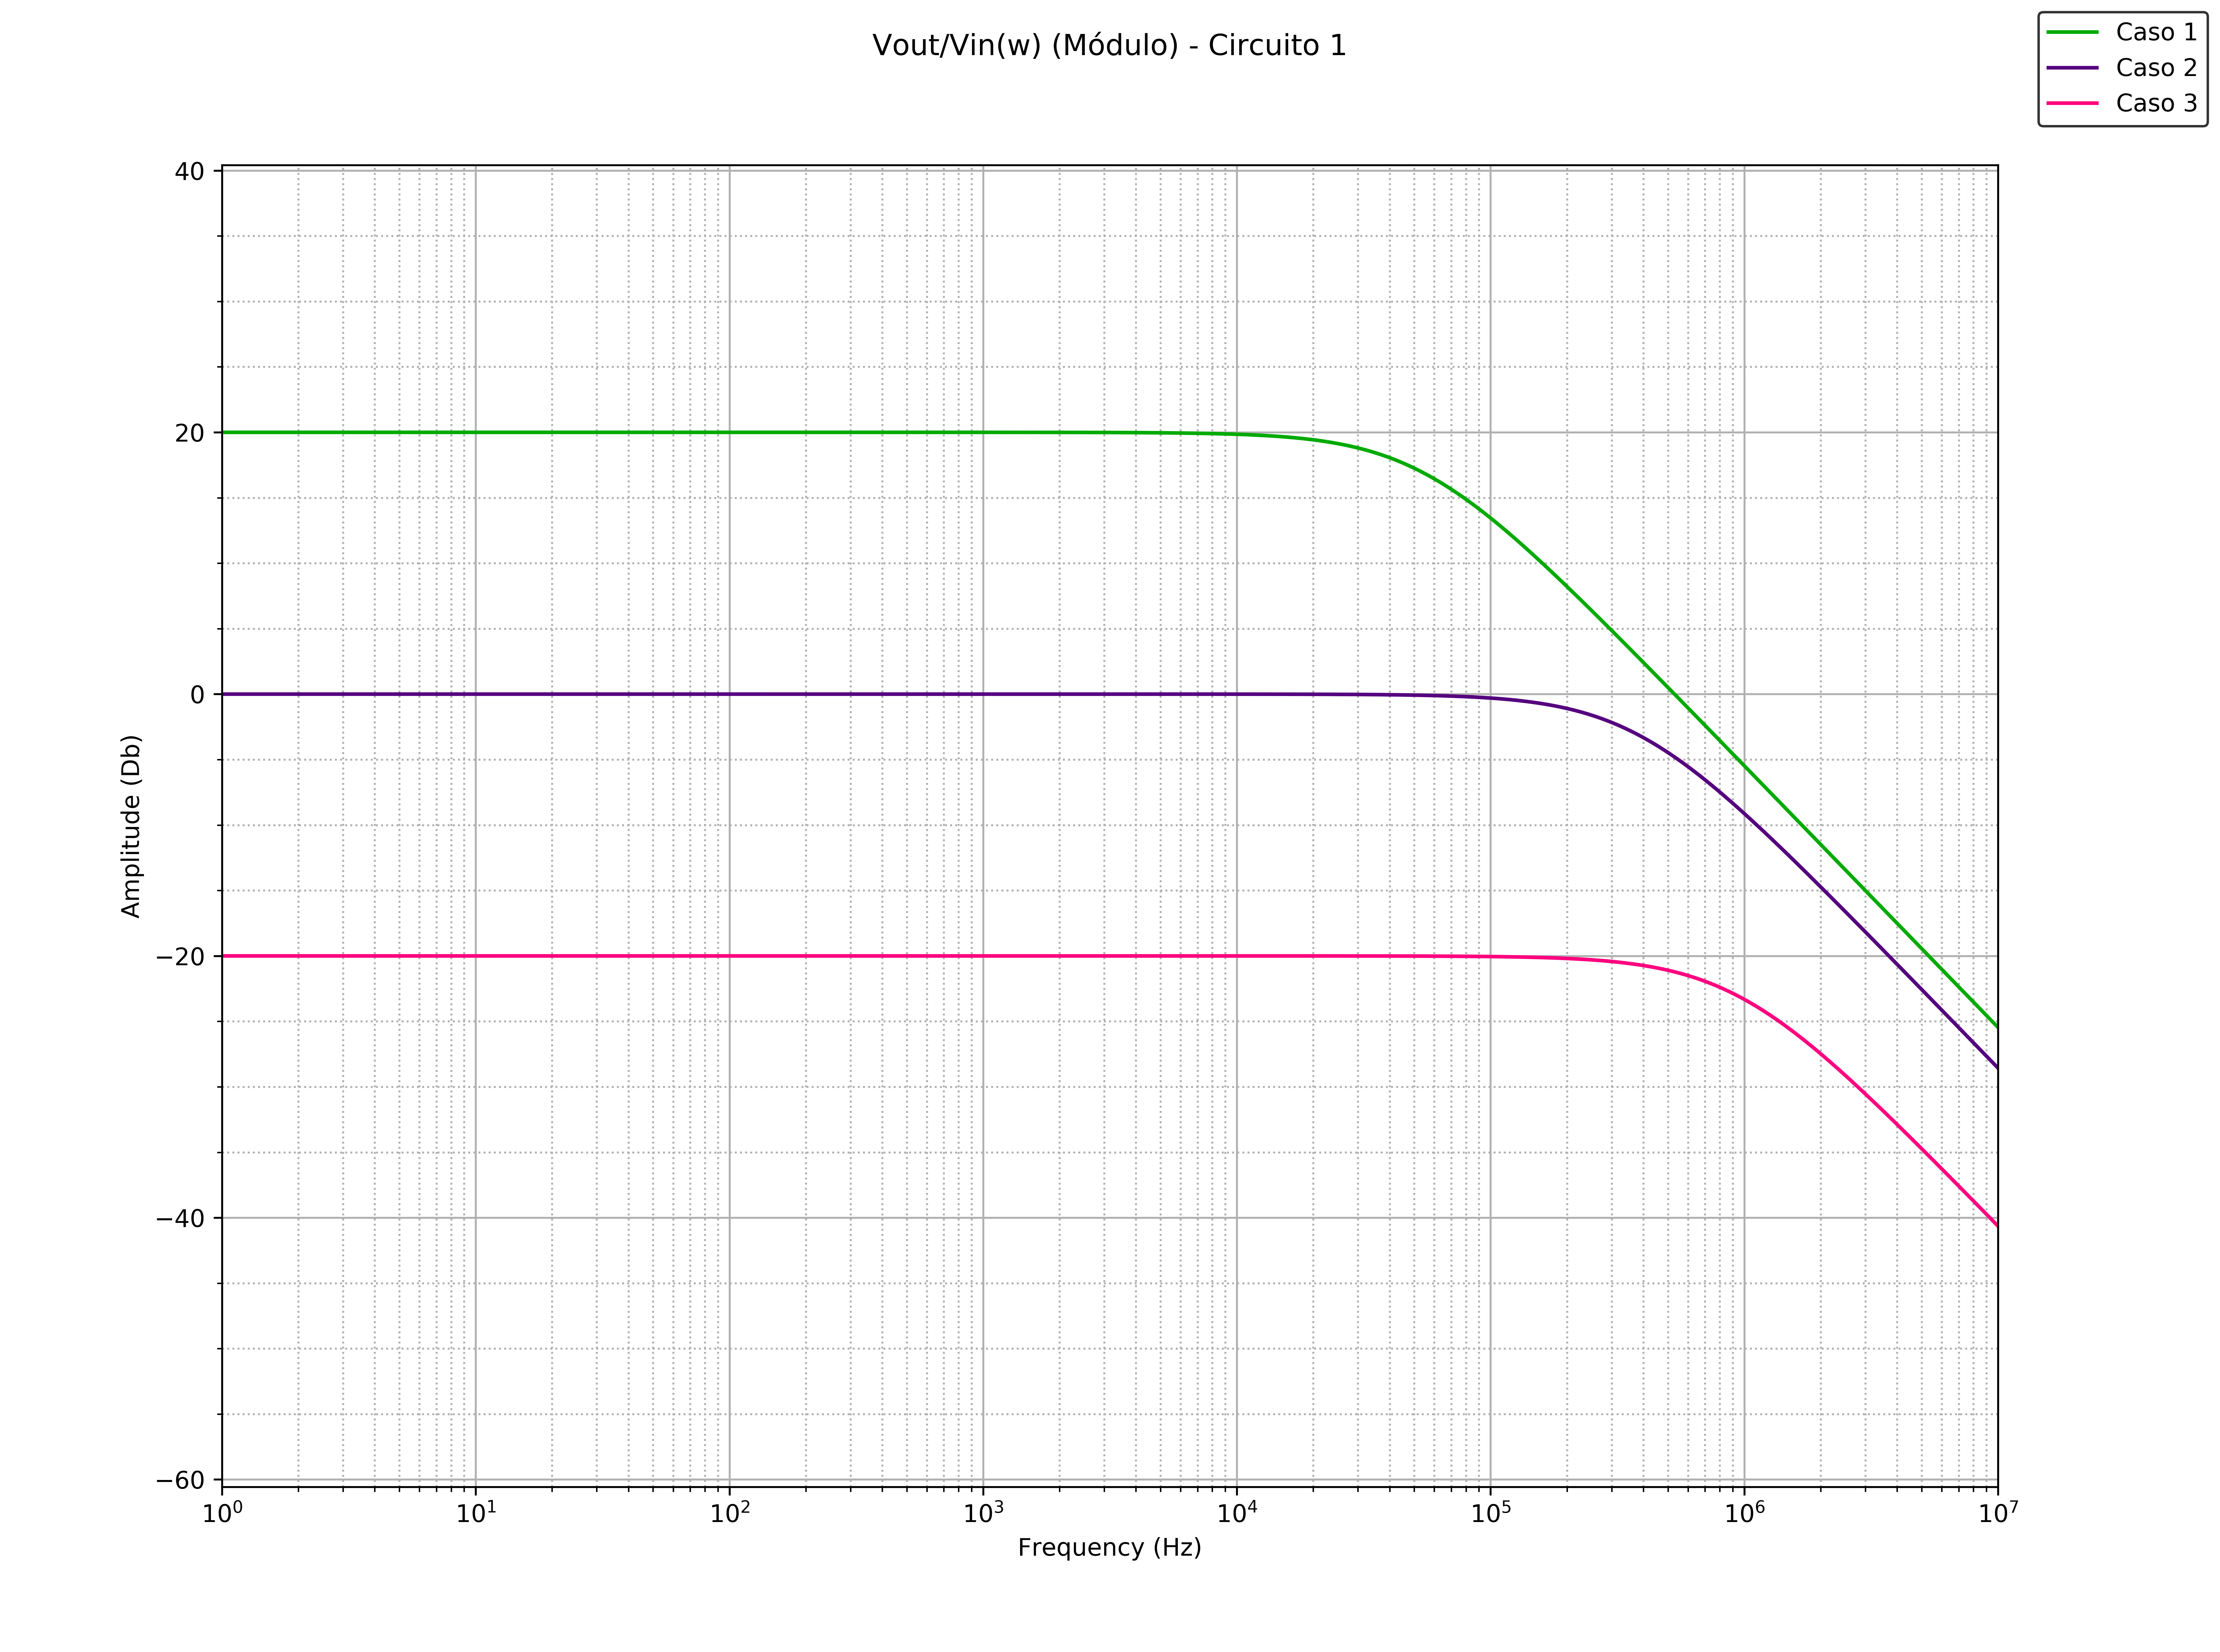
\includegraphics[width=10cm,height=10cm,keepaspectratio]{../EJ1/00GRAFICOS/teoricos/circ1voviw.png}
	\caption{Configuración inversora - Comparaci\'on te\'orica del m\'odulo de $V_{out}/V_{in}$ para los tres casos.}
	\label{c1voviTeoMod}
\end{figure}

\begin{figure}[H] %!ht
	\centering
	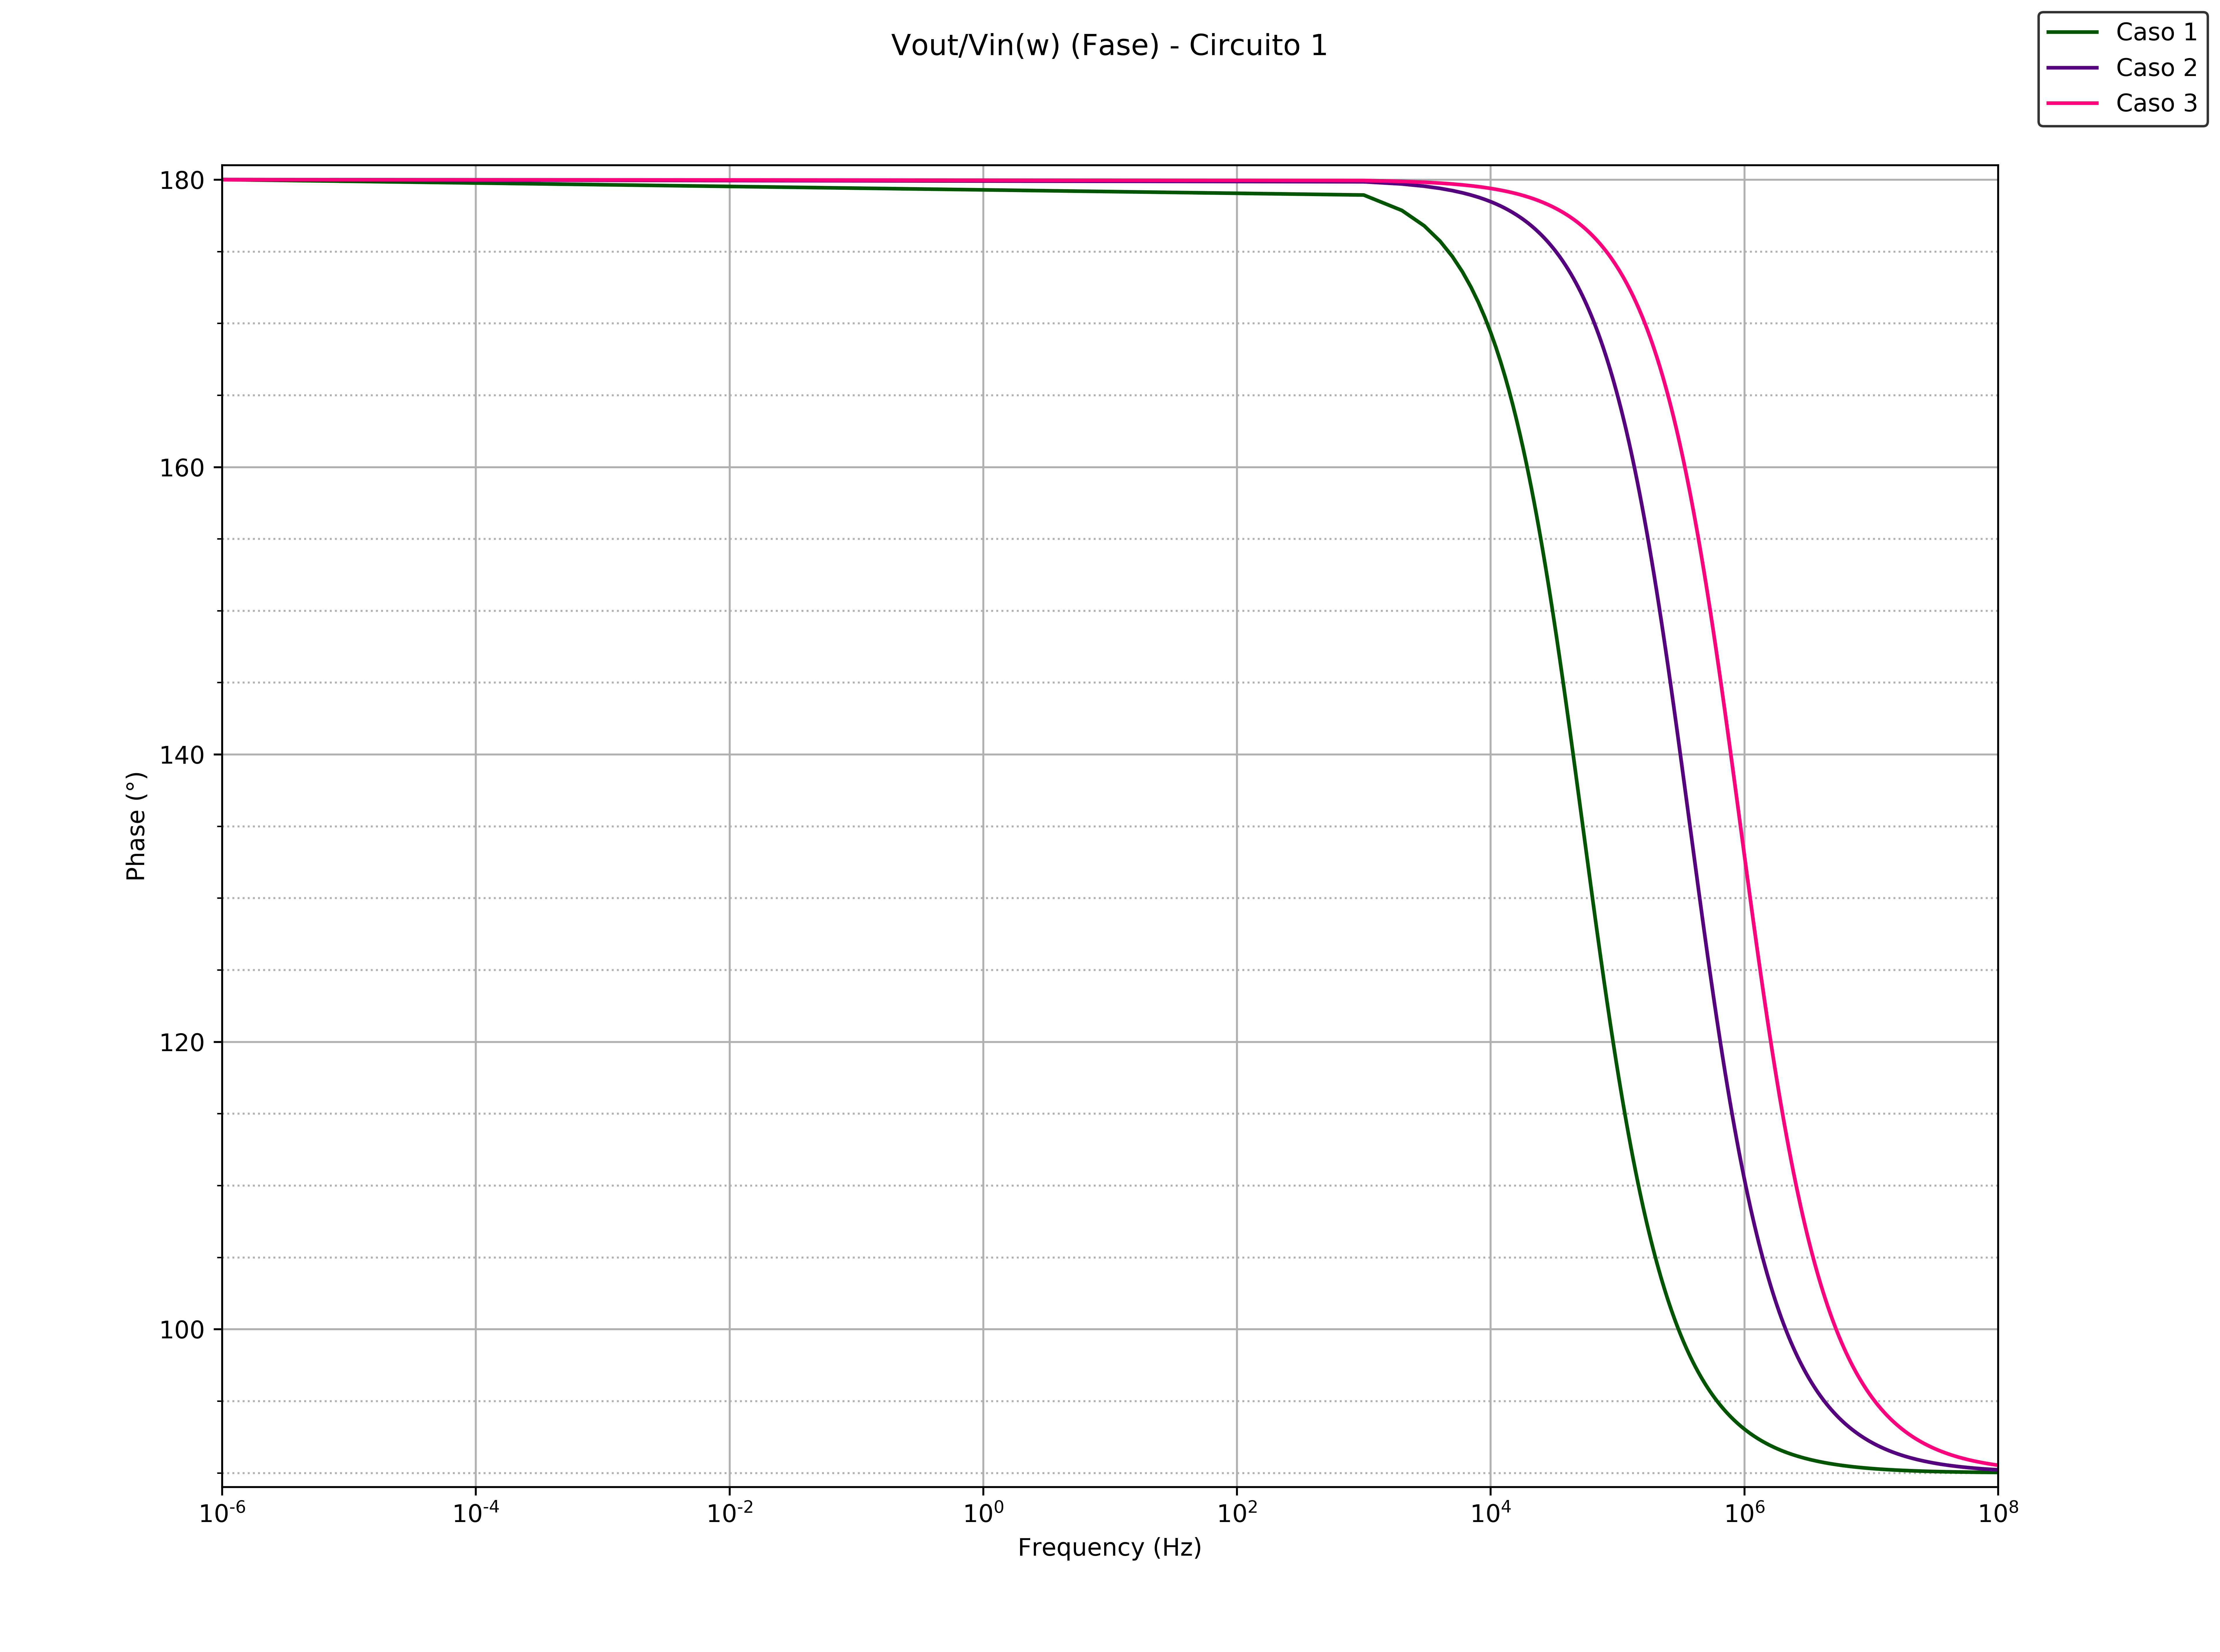
\includegraphics[width=10cm,height=10cm,keepaspectratio]{../EJ1/00GRAFICOS/teoricos/circ1vovifasew.png}
	\caption{Configuración inversora - Comparaci\'on te\'orica de la fase de $V_{out}/V_{in}$ para los tres casos.}
	\label{c1voviTeoPh}
\end{figure}

El gr\'afico \ref{c1voviTeoMod} permite ver una caracter\'istica importante que diferencia a los tres casos de 
resistencias para este circuito: la ganancia a bajas frecuencias. Las tres configuraciones corresponden 
a filtros pasabajos. Si bien aten\'uan a altas frecuencias, 
tienen comportamientos diferentes en las frecuencias bajas. 
Aqu\'el con resistencias para el caso 1 presenta una ganancia de 20dB, 
mientras que el del caso 3 aten\'ua 20 dB. El circuito del caso 2, por el contrario, no gana ni aten\'ua 
en frecuencias bajas. A bajas frecuencias, lo que se observa en el gr\'afico \ref{c1voviTeoMod} coincide con los valores presentados previamente en la tabla \ref{avolf} (los cuales fueron hechos para el caso de frecuencia cero.


%%%%%%%%%%%%%%%%%%%%%%%%%%%%%%%%%%%%%%%%%%%%%%%%%%%%%%%%%%%%%%%%%%%%%%%%%
\subsubsection*{Configuraci\'on no inversora}

Para el circuito \ref{c2} se parte de las siguientes ecuaciones, similares a las del an\'alisis del circuito inversor. 

\begin{equation}
	\begin{cases}
		V_{out} = A_{vol}\cdot(V^+ - V^-) \\
		V_{in} - R_3 \cdot I_3 = V^+ \\
		V_{out} - R_2 \cdot I_2 = V^- \\
		I_4 = I_3\\
		I_2 = I_1
	\end{cases}
	\label{ecsbase2}
\end{equation}



Operando matem\'aticamente, se obtiene la siguiente expresi\'on:

\begin{equation}
	\frac{V_{out}}{V_{in}} =  \frac{A_{vol} \cdot R_4 \cdot (R_1 + R_2)}{(R_3 + R_4) \cdot (R_1 + R_2 + A_{vol} \cdot R_1)}
	\label{c2vovi}
\end{equation}

Al igual que para el circuito inversor, a continuaci\'on se muestran
los resultados obtenidos al evaluar la ecuaci\'on \ref{c2vovi} con las resistencias
de cada caso y considerando $A_{vol}$ finito.

\begin{table}[h!]
	\centering
	\begin{tabular}{c c c}%
		\bfseries  & $V_{out}/V_{in}$ &  $|V_{out}/V_{in}| (dB)$\\ \hline
		caso 1 & $8,799$ & $18,889$ \\
		caso 2 & $1,600$ & $4,082$\\
		caso 3 & $8,800$ & $18,889$\\
		\hline
	\end{tabular}
	\caption{$V_{out}/V_{in}$ del circuito inversor considerando $A_{vol}$ finito.}
	\label{avolf2}
\end{table}

A diferencia que para el circuito inversor, se puede notar que
 los valores de $V_{out}/V_{in}$ son positivos, lo cual concuerda con que se trata de un circuito no inversor. En este circuito los casos 1 y 3 presentan la misma ganancia de casi $19dB$ al considerar $A_{vol}$ finito, mientras que el caso 2 tambi\'en presenta ganancia, pero menor (de 4dB).


Por otro lado, reemplazando con los valores de resistencias correspondientes
 a cada caso y con $A_{vol}(\omega)$, se obtiene:

Caso1:-
\begin{equation}
	\frac{V_{out}}{V_{in}} = \frac{22 \cdot 10^8}{437,68 s + 25 \cdot 10^7}
	\label{c2c1vovi}
\end{equation}

caso 2:
\begin{equation}
	\frac{V_{out}}{V_{in}} = \frac{4 \cdot 10^8}{79,577 s + 25 \cdot 10^7}
	\label{c2c2vovi}
\end{equation}

caso 3:
\begin{equation}
	\frac{V_{out}}{V_{in}} = \frac{22 \cdot 10^8}{437,68 s + 25 \cdot 10^8}
	\label{c2c3vovi}
\end{equation}

En los gr\'aficos que se muestran a continuaci\'on (\ref{c2voviTeoMod} y \ref{c2voviTeoPh}) pueden verse los resultados de estos c\'alculos.

\begin{figure}[H] %!ht
\centering
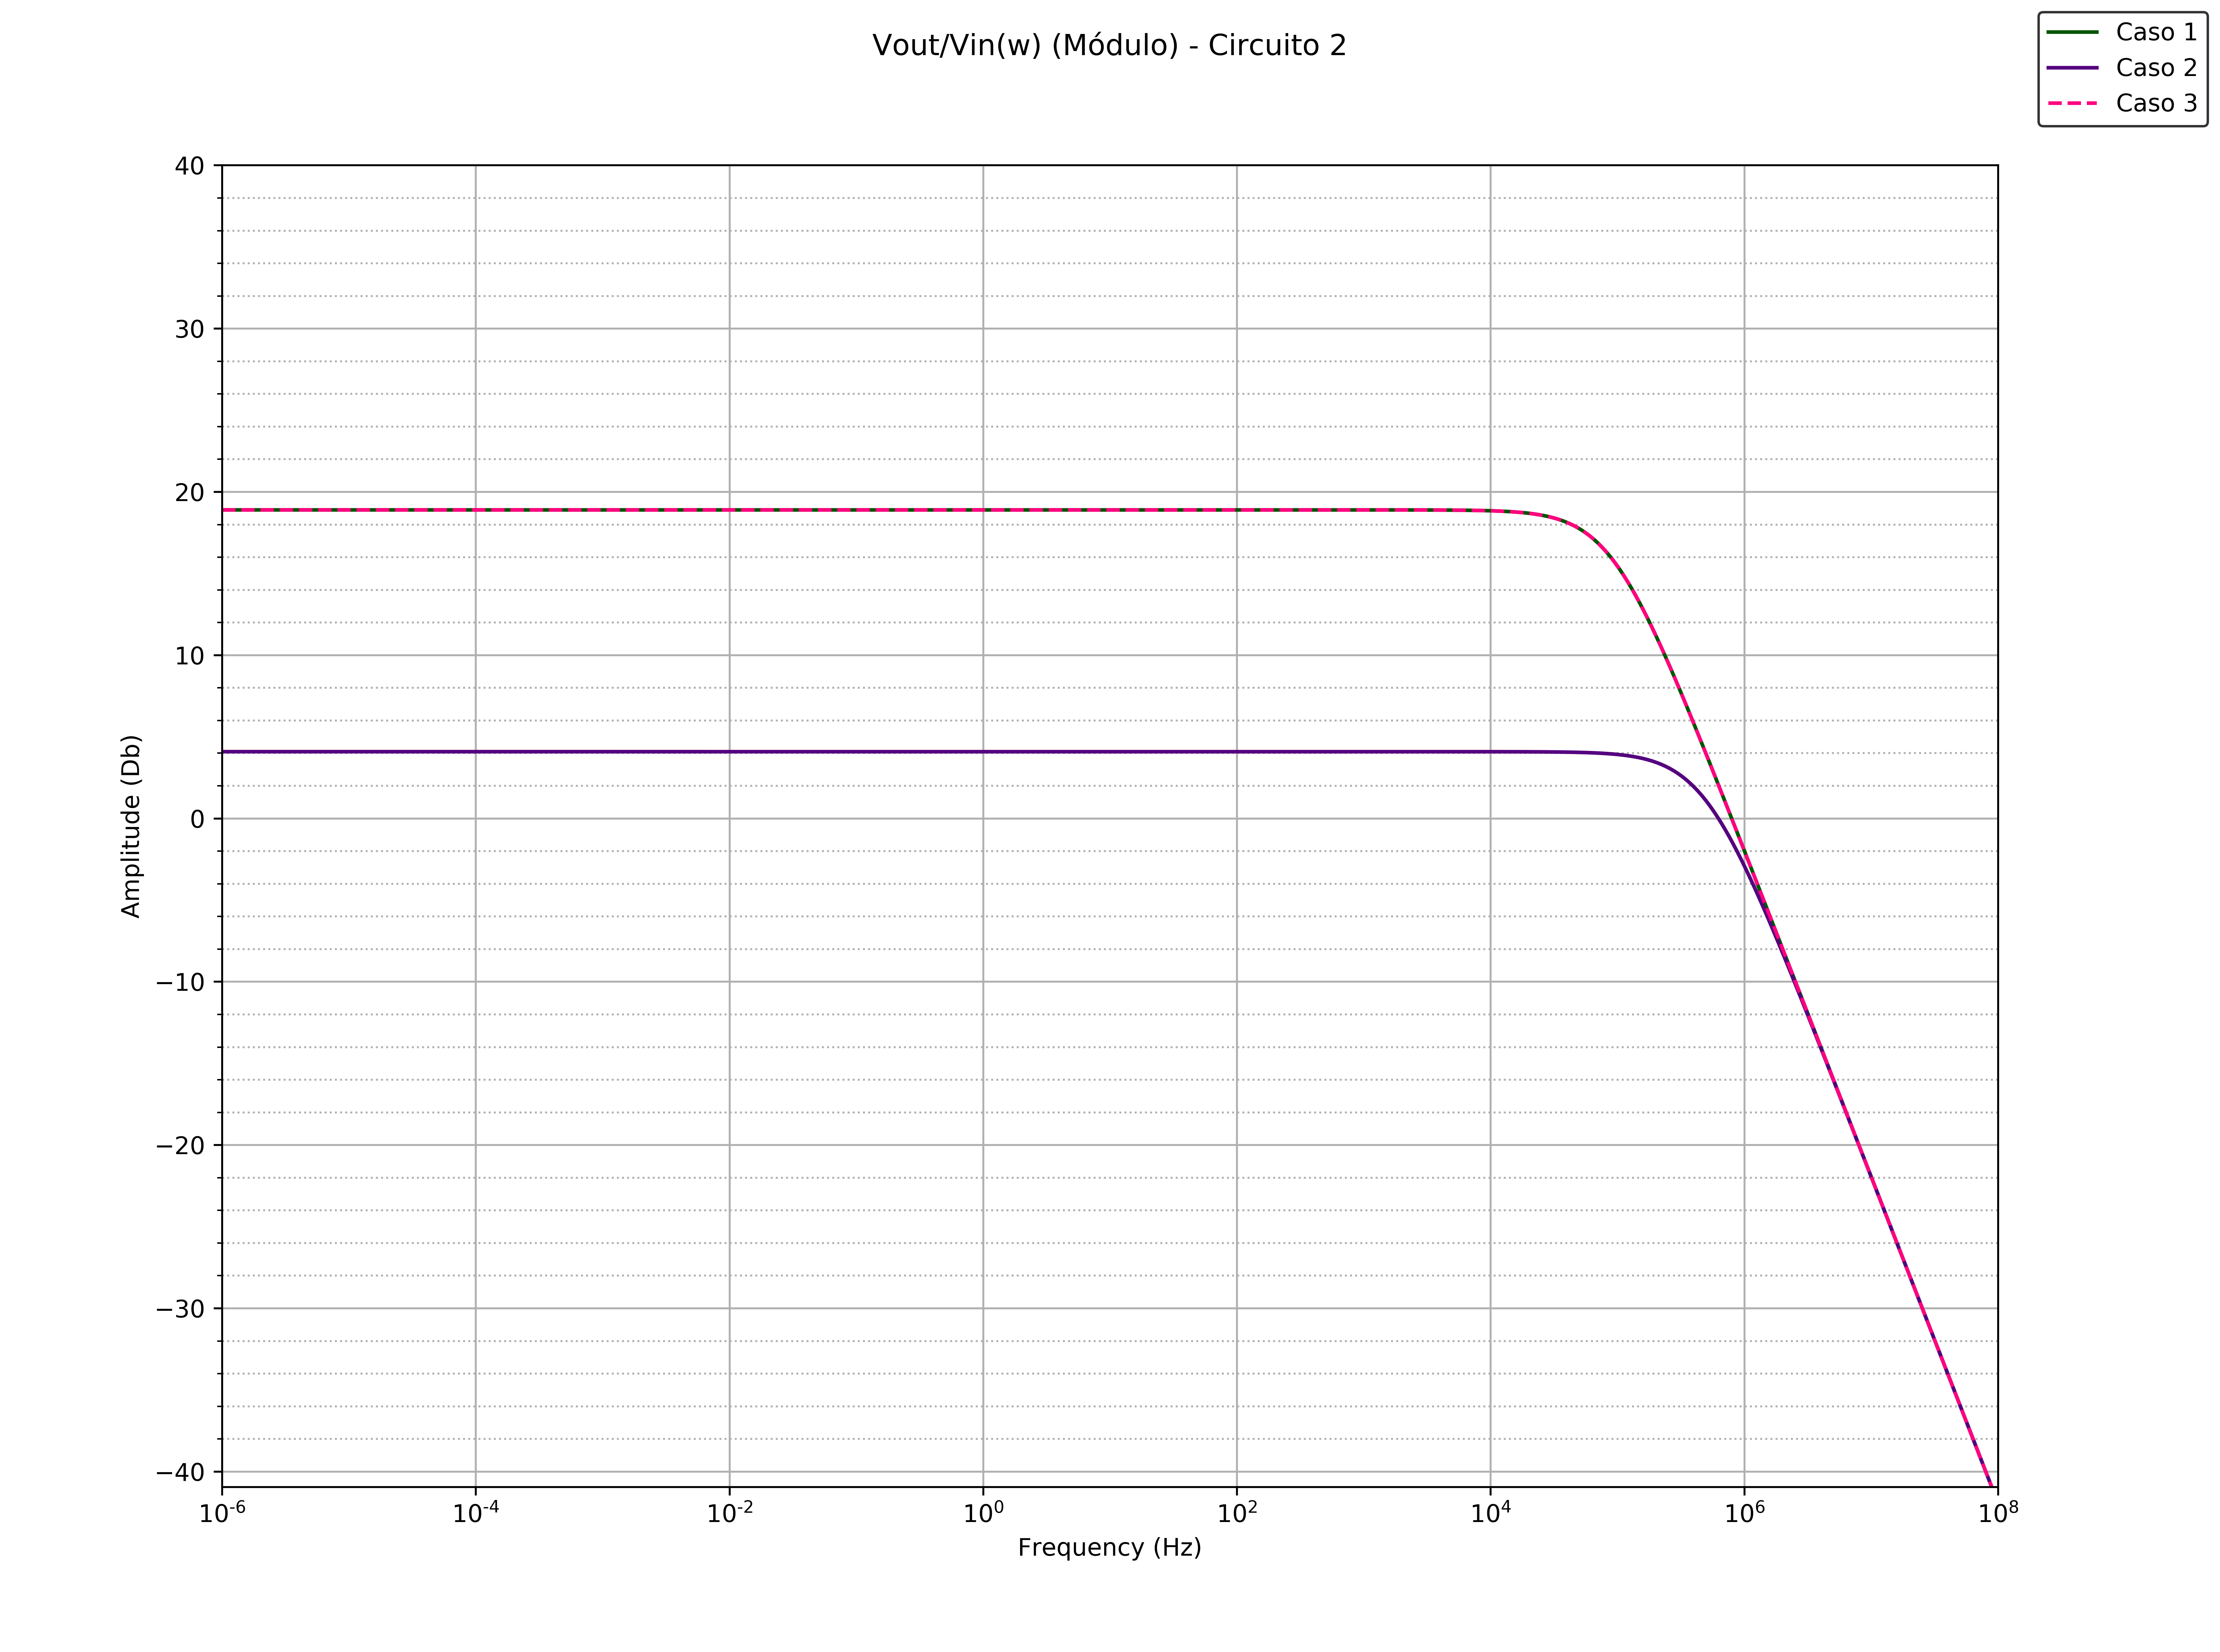
\includegraphics[width=10cm,height=10cm,keepaspectratio]{../EJ1/00GRAFICOS/teoricos/circ2voviw.png}
\caption{Configuración no inversora - Comparaci\'on te\'orica del m\'odulo de$V_{out}/V_{in}$ de los tres casos.}
\label{c2voviTeoMod}
\end{figure}

\begin{figure}[H] %!ht
\centering
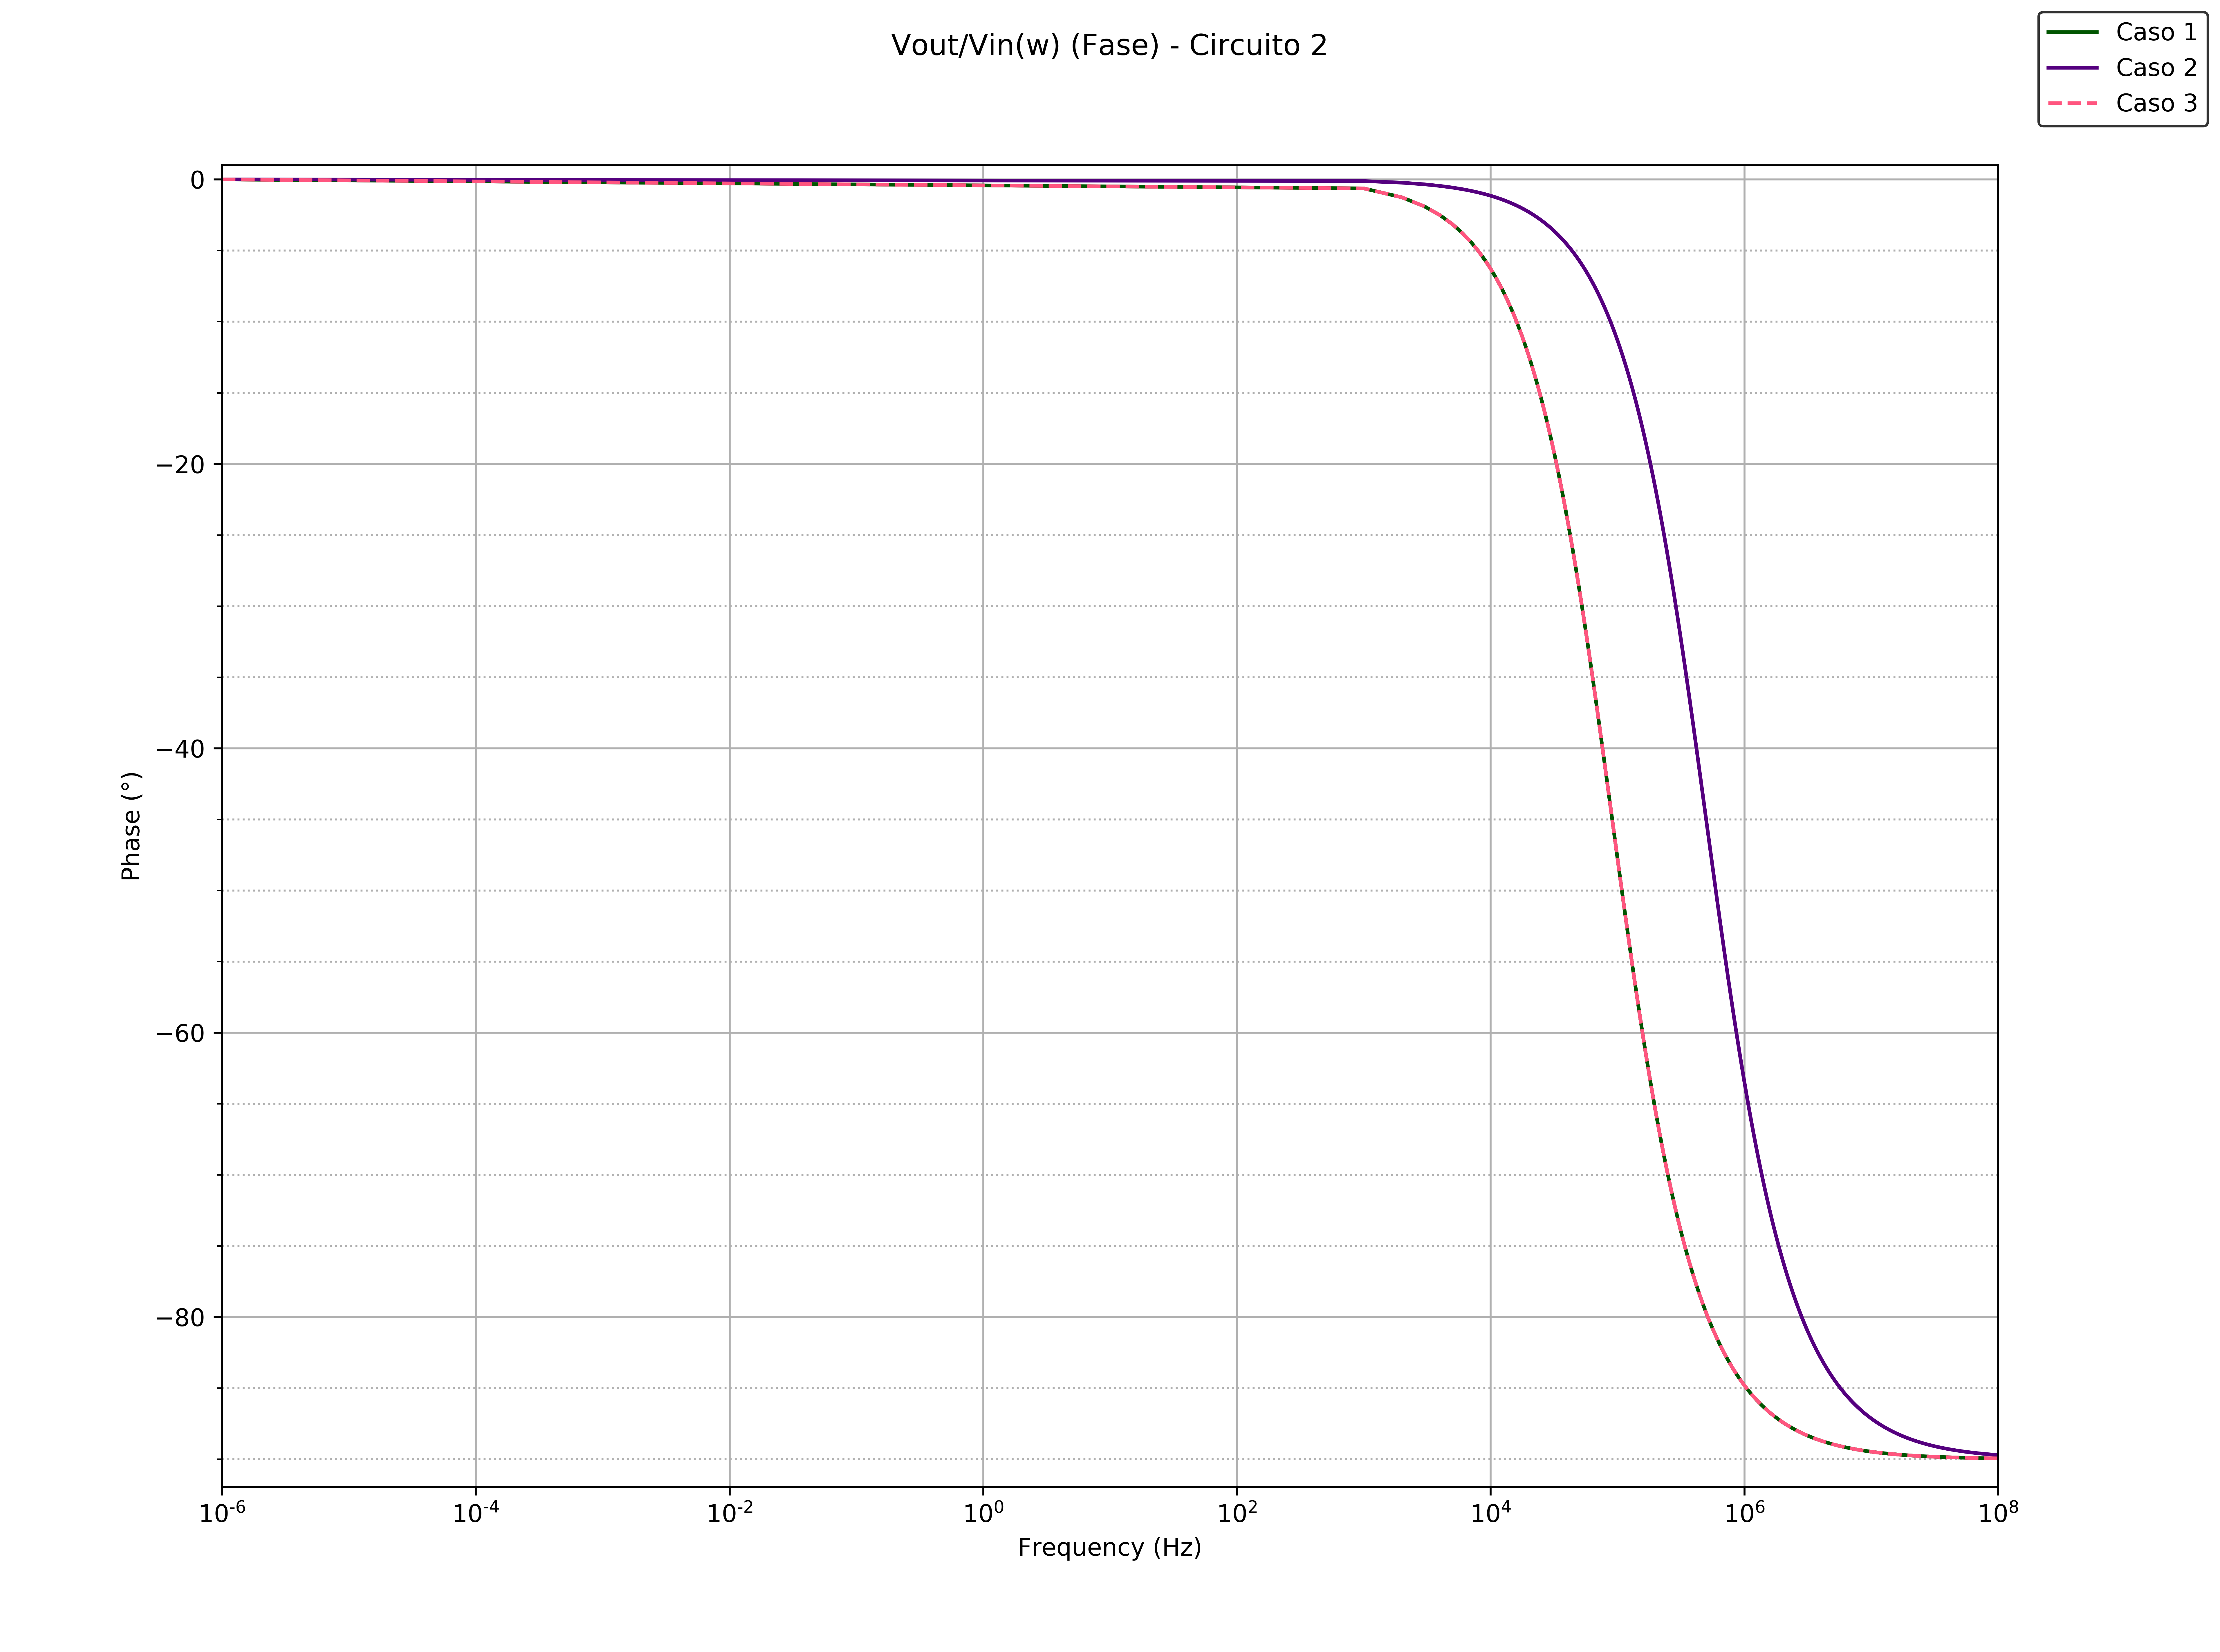
\includegraphics[width=10cm,height=10cm,keepaspectratio]{../EJ1/00GRAFICOS/teoricos/circ2vovifasew.png}
\caption{Configuración no inversora - Comparaci\'on te\'orica de la fase de $V_{out}/V_{in}$ de los tres casos.}
\label{c2voviTeoPh}
\end{figure}

Puede verse en el gr\'afico \ref{c2voviTeoMod} que a bajas frecuencias los valores de ganancias coinciden con los calculados para $A_{vol}$ finito. Al ser este gr\'afico en funci\'on de la frecuencia, permite observar que el no inversor tambi\'en se comporta como un filtro pasa bajos atenuando las altas frecuencias.






\subsubsection{Mediciones y resultados obtenidos} %%%%%%%

La respuesta en frecuencia es una herramienta de análisis útil para todo circuito. Se estimuló a los seis circuitos con una se\~nal senoidal de frecuencia variable, realizando un barrido por el espectro de frecuencias que consideramos relevante, en función a las simulaciones realizadas en LTSpice. Para cada valor de frecuencia se observó la diferencia de fase y la relación de amplitudes entre la se\~nal de entrada y la salida de los circuitos, conformando un diagrama de BODE completo. Se superpusieron dichas mediciones con las simulaciones, obteniendo los siguientes gráficos.
Cabe destacar que la medición estuvo altamente influida por fenómenos tales como el “crossover distortion” y el “slew rate” los cuales se desarrollarán a continuación.
\subsubsection*{Configuraci\'on inversora}
Se simul\'o y se midi\'o la ganancia para los tres casos del circuito \ref{c1} 
y a continuacio\'on se puede ver la diferencia entre sus resultados y los 
de las ecuaciones \ref{c1c1vovi}, \ref{c1c2vovi} y \ref{c1c3vovi}; correspondientes a 
la ganancia calculada de forma te\'orica y considerando al amplificador operacional como ideal.


\begin{figure}[H] %!ht
	\centering
	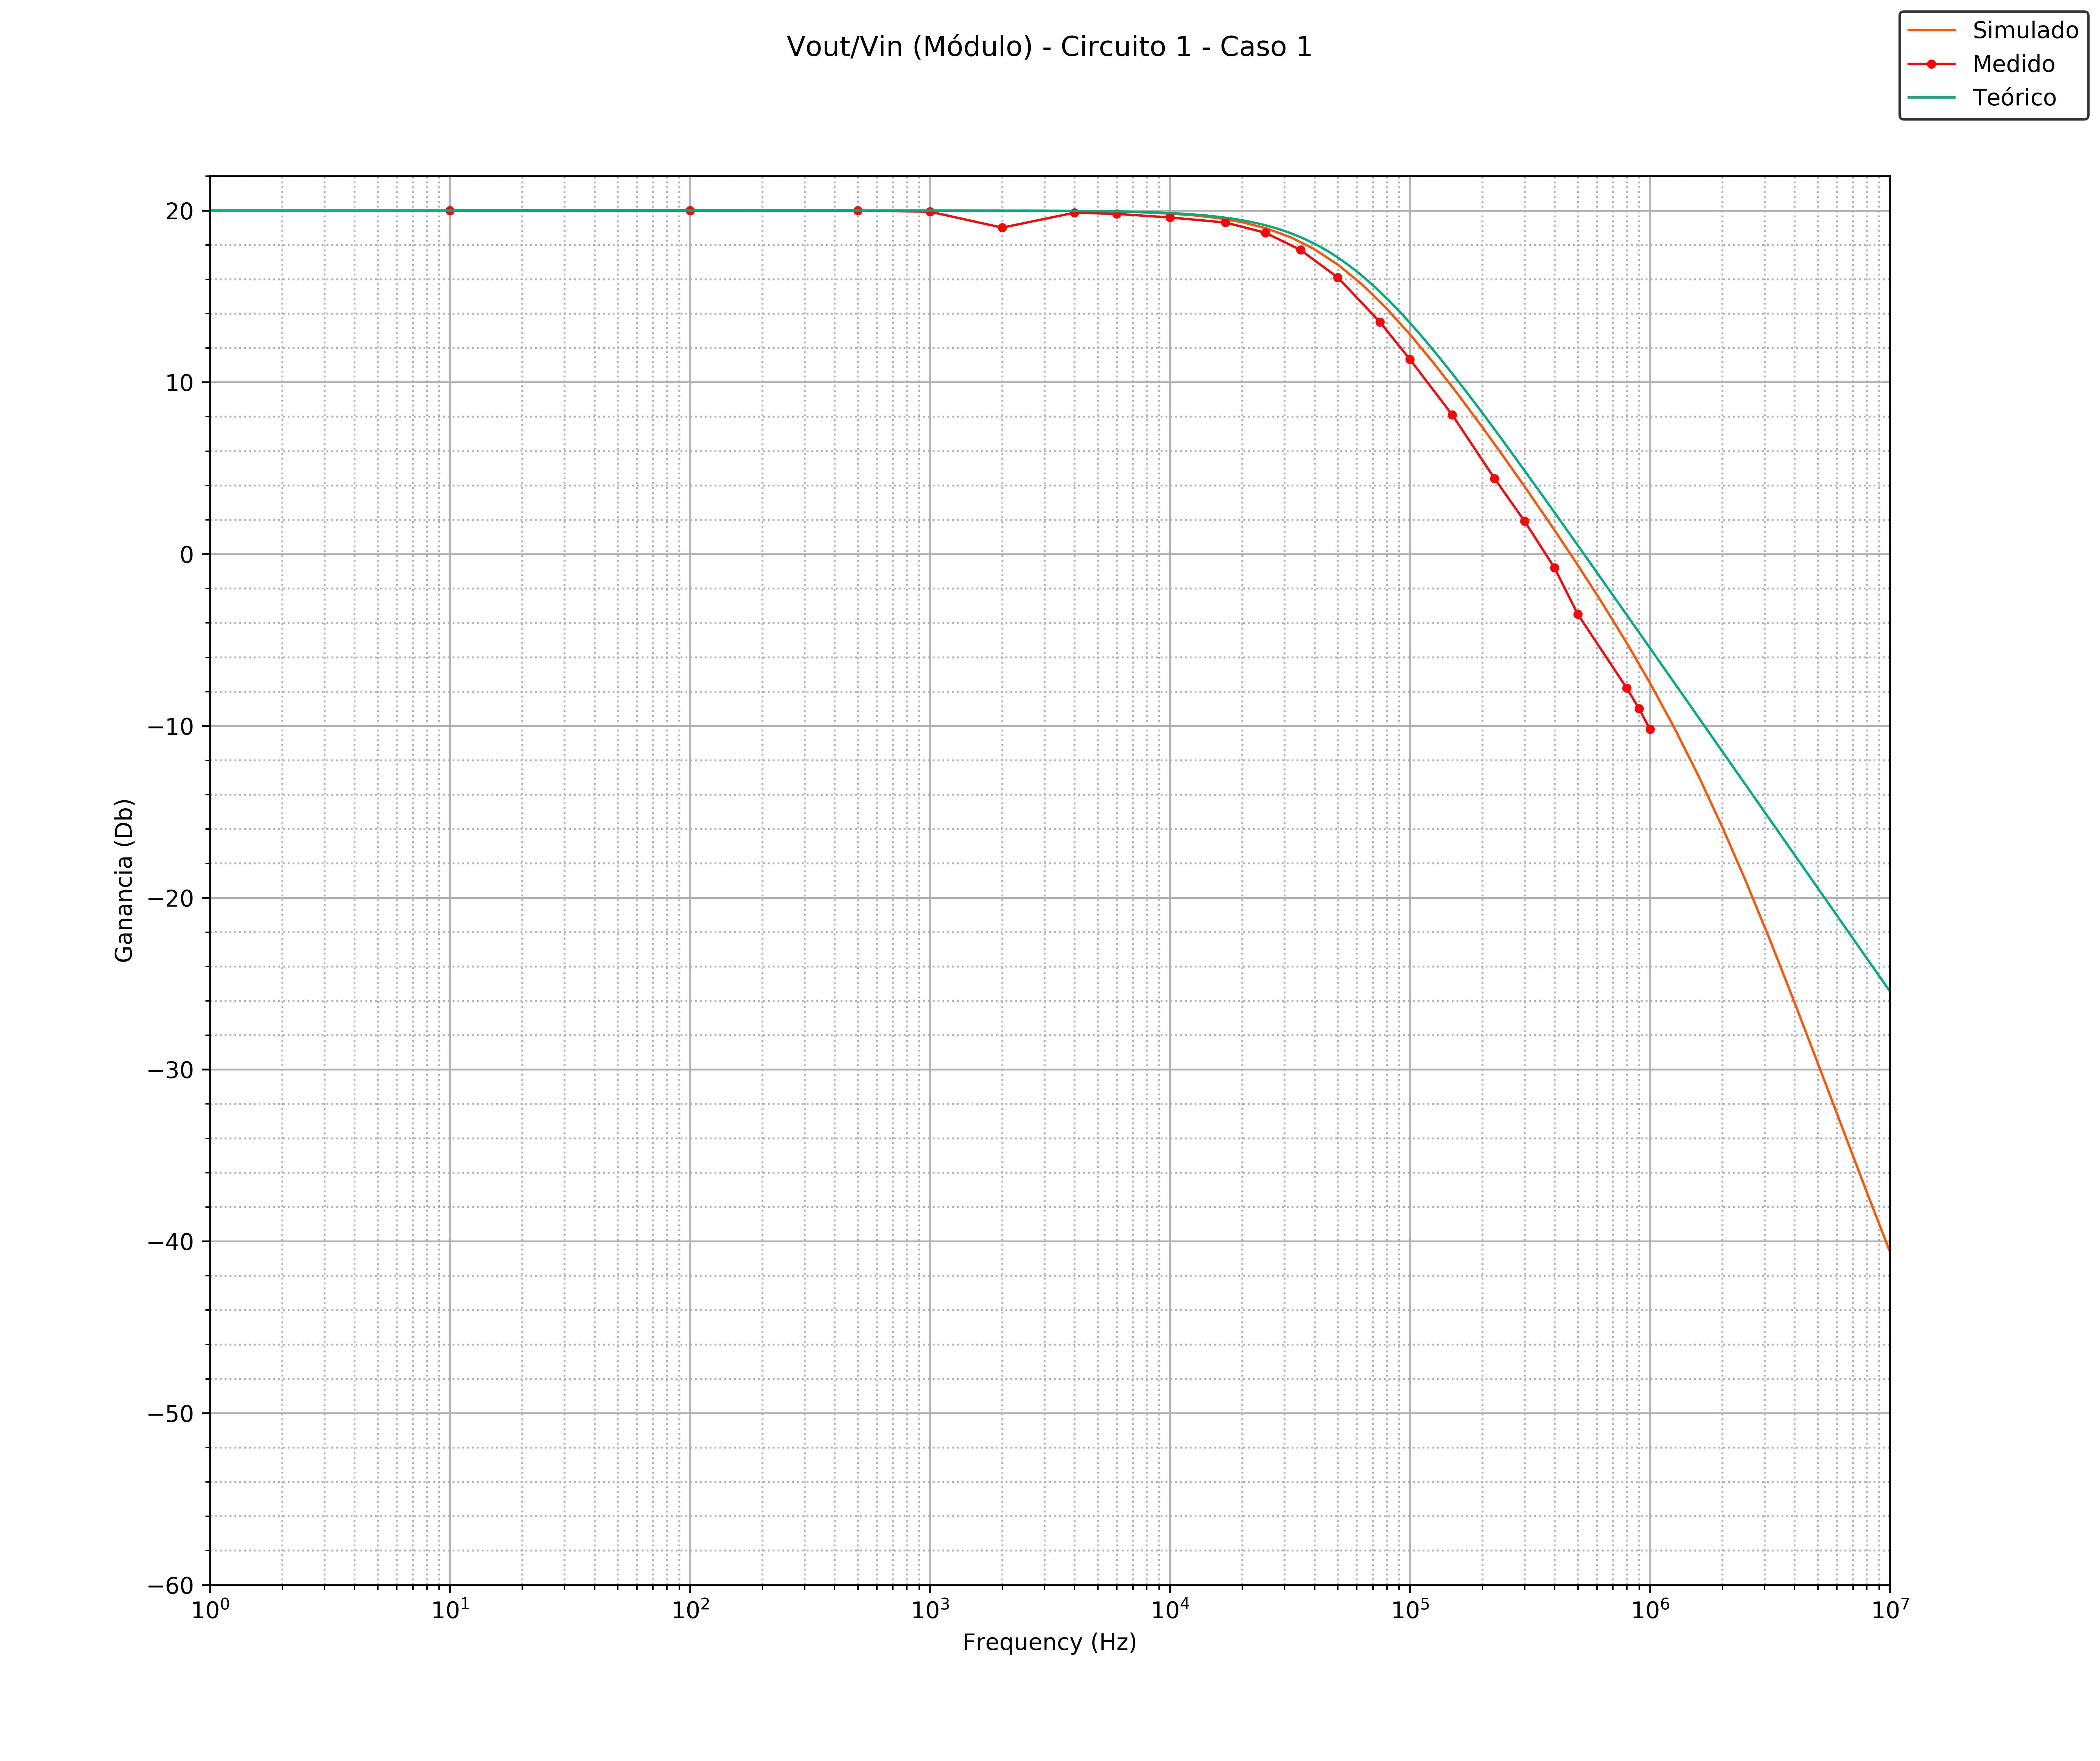
\includegraphics[width=10cm,height=10cm,keepaspectratio]{../EJ1/00GRAFICOS/c1c1/c1c1voviMod.png}
	\caption{Configuración inversora -  Caso 1 - Módulo de $V_{out}/V_{in}$}
	\label{c1c1voviM}
\end{figure}

\begin{figure}[H] %!ht
	\centering
	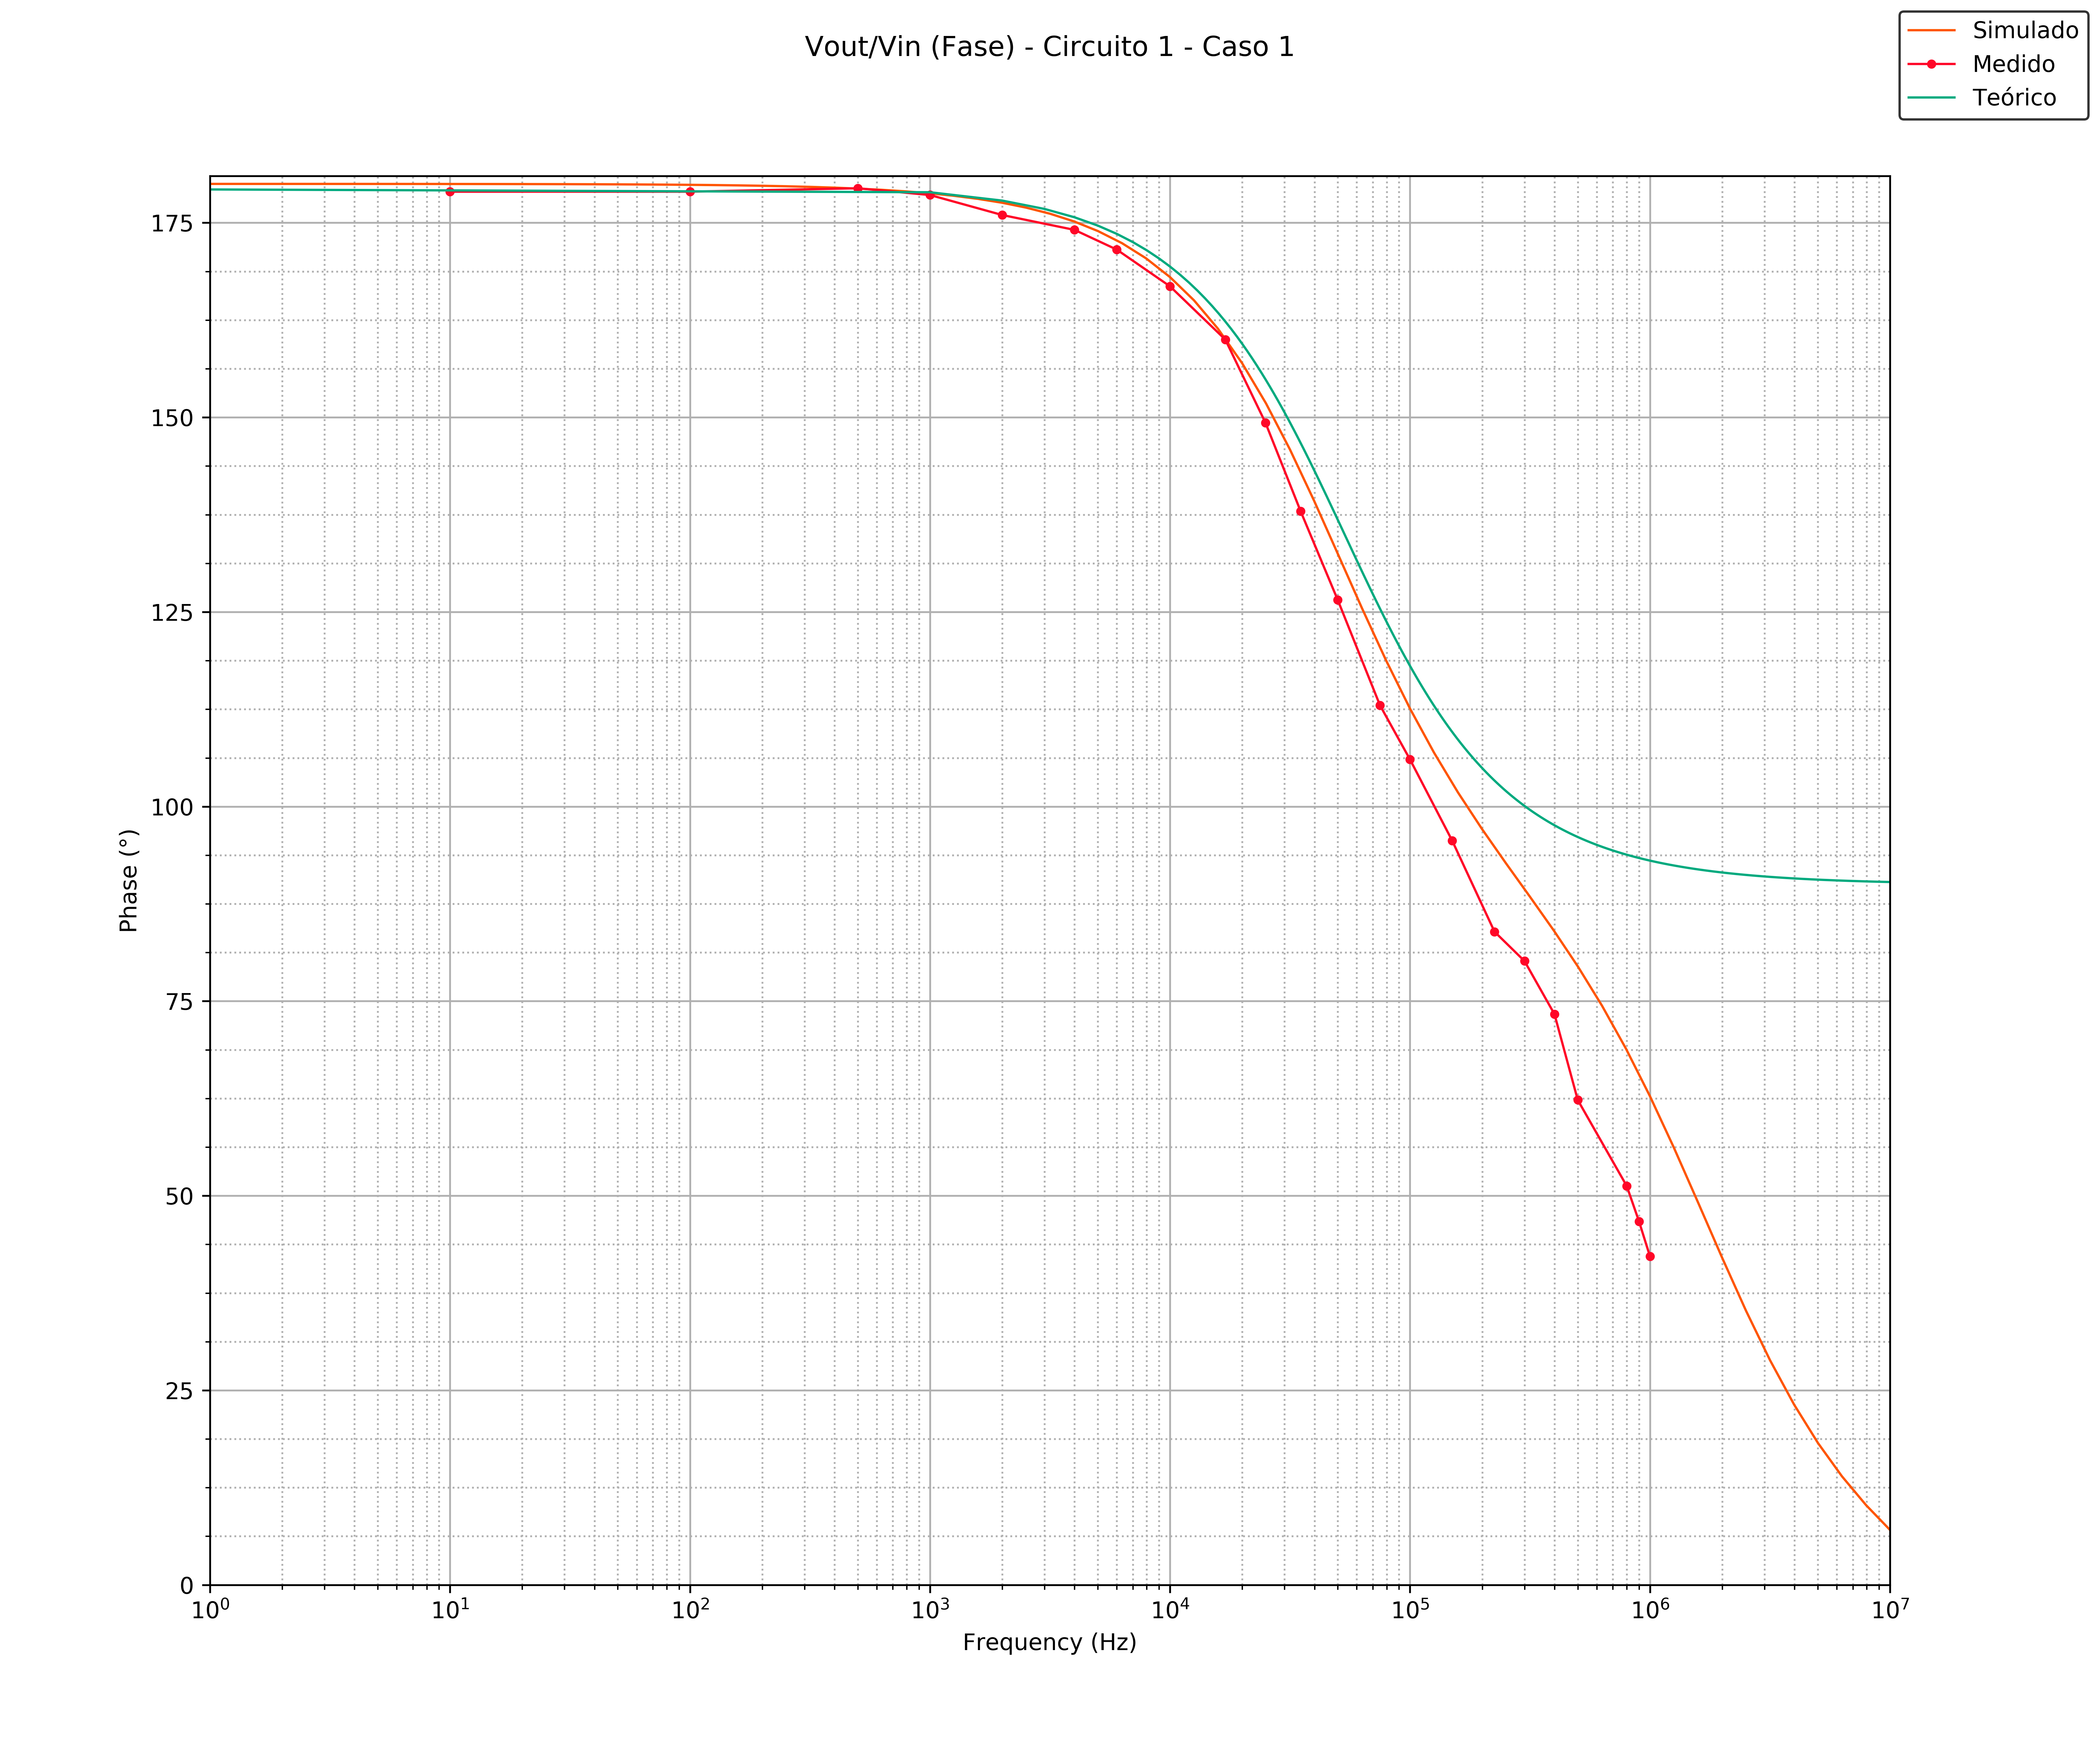
\includegraphics[width=10cm,height=10cm,keepaspectratio]{../EJ1/00GRAFICOS/c1c1/c1c1voviFASE.png}
	\caption{Configuración inversora - Caso 1 - Fase de $V_{out}/V_{in}$}
	\label{c1c1voviP}
\end{figure}

\begin{figure}[H] %!ht
	\centering
	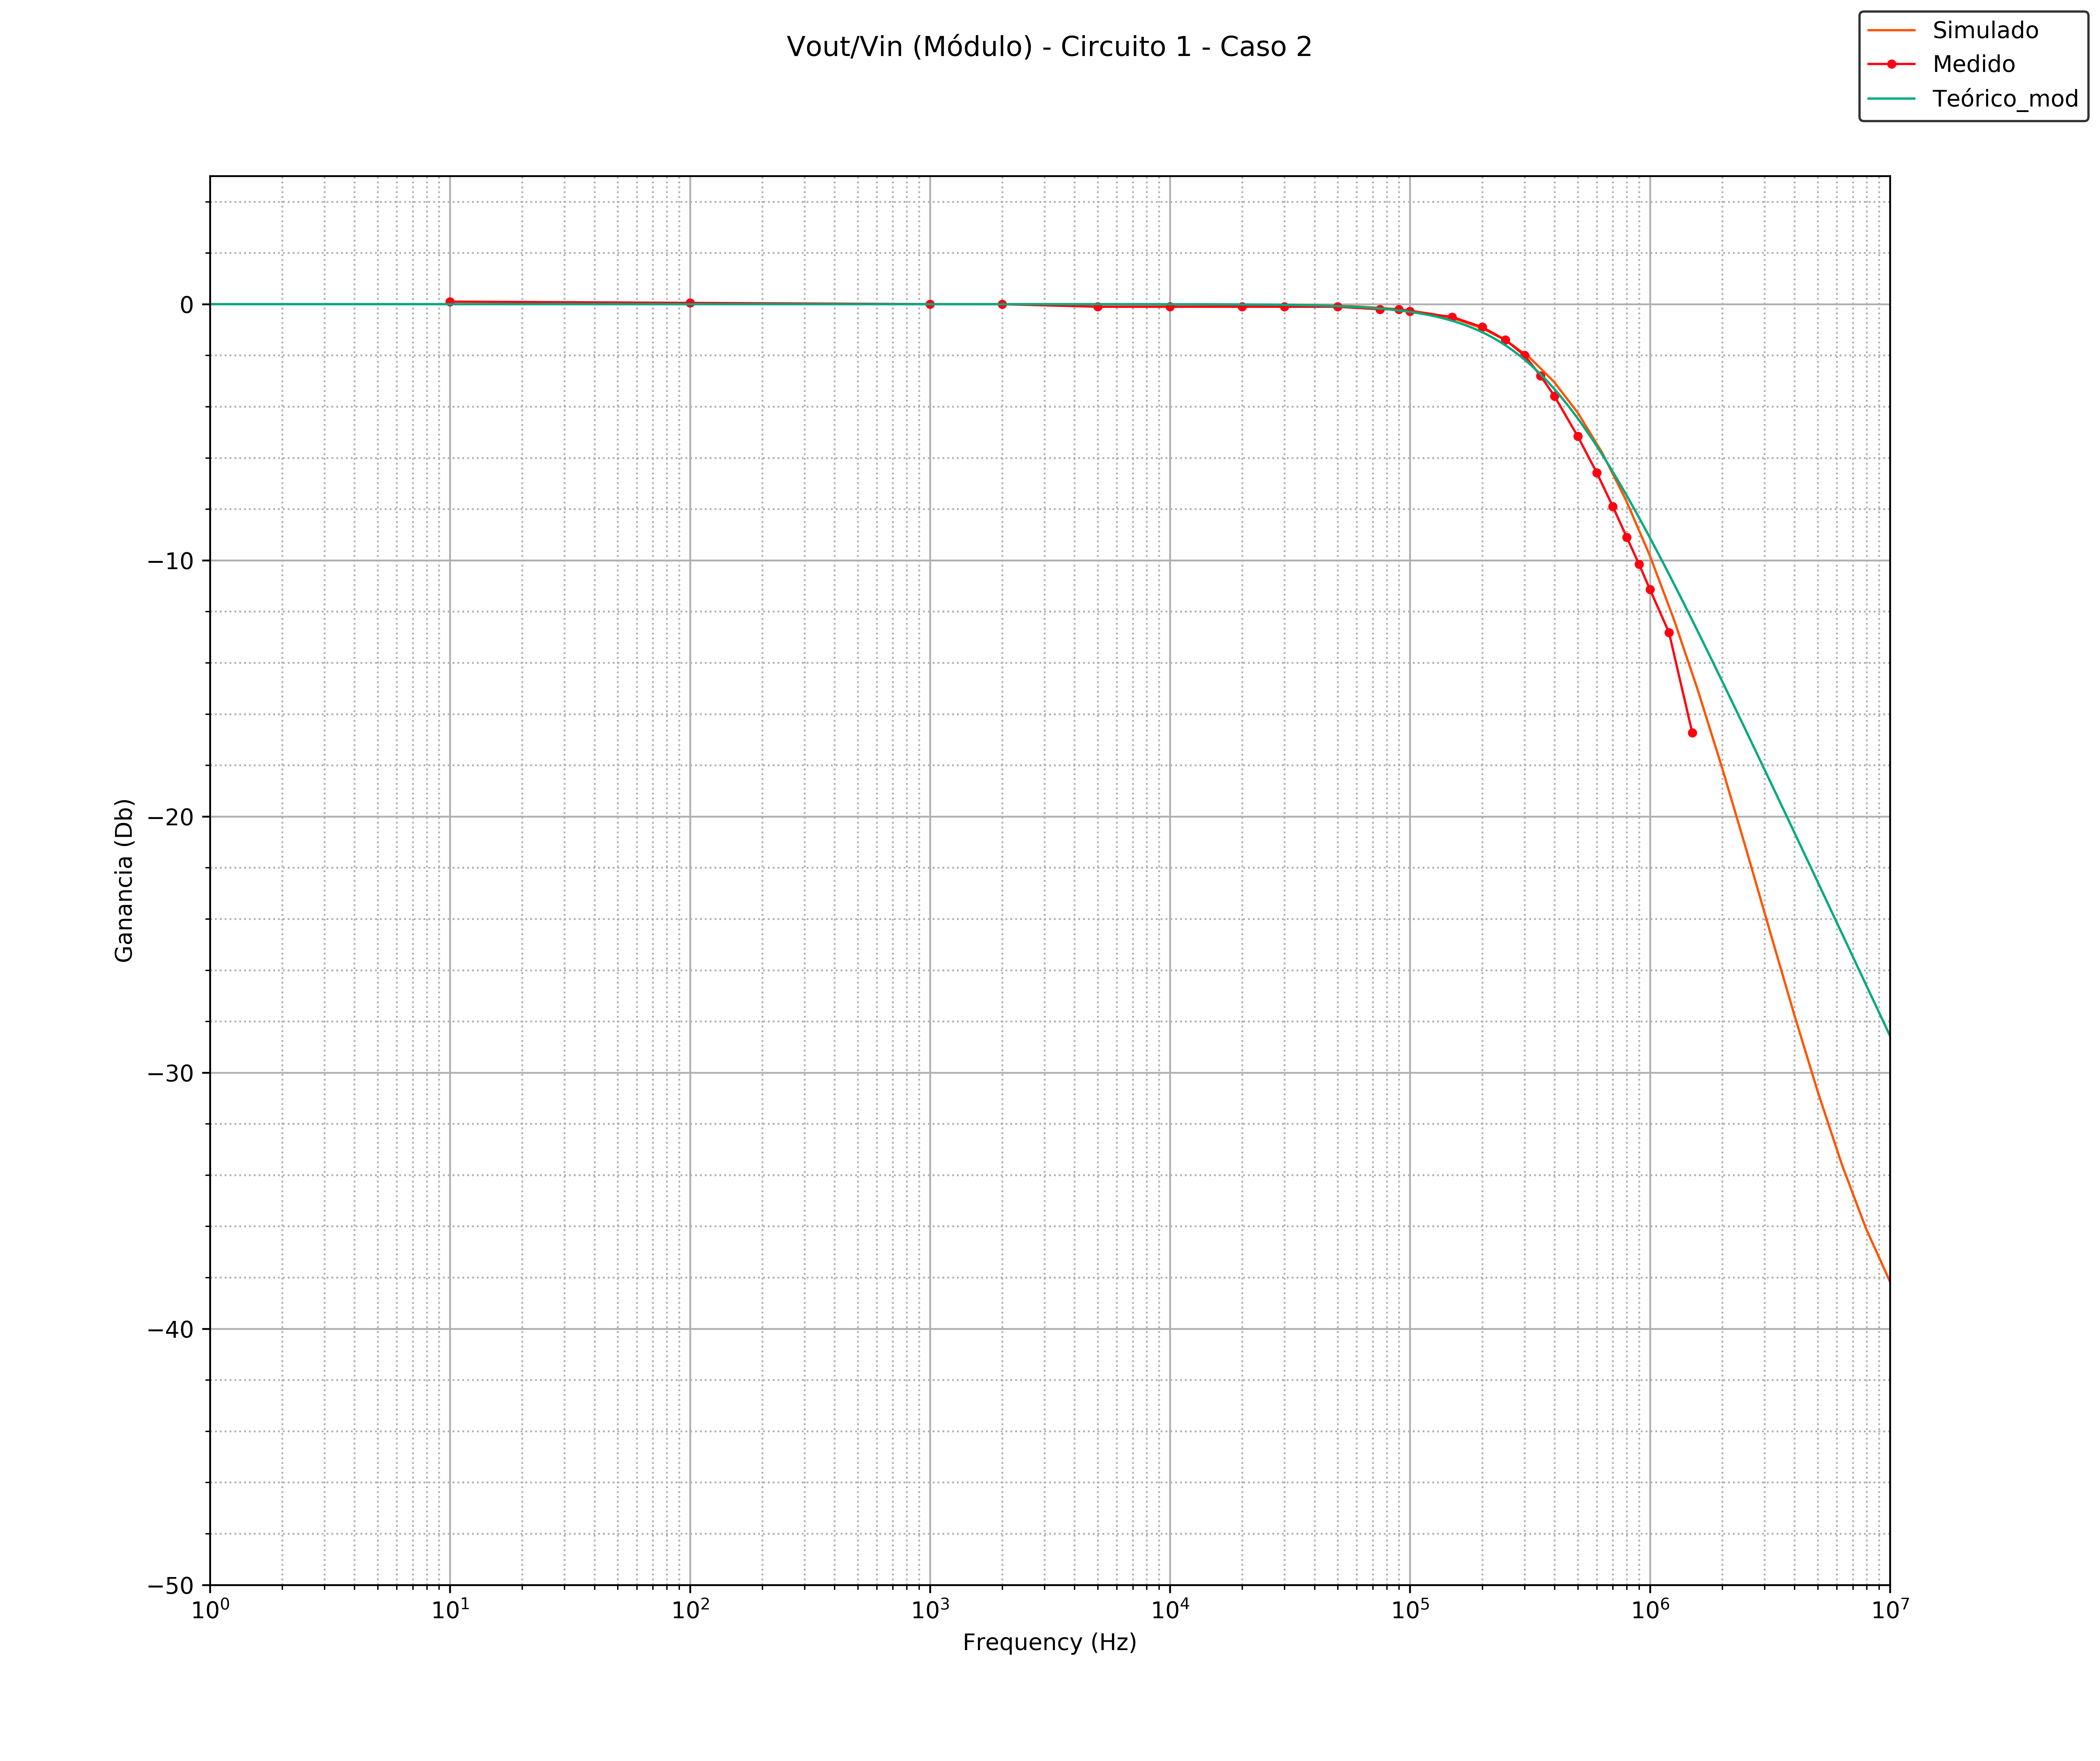
\includegraphics[width=10cm,height=10cm,keepaspectratio]{../EJ1/00GRAFICOS/c1c2/c1c2voviMod.png}
	\caption{Configuración inversora - Caso 2 - Módulo de $V_{out}/V_{in}$}
	\label{c1c2voviM}
\end{figure}

\begin{figure}[H] %!ht
	\centering
	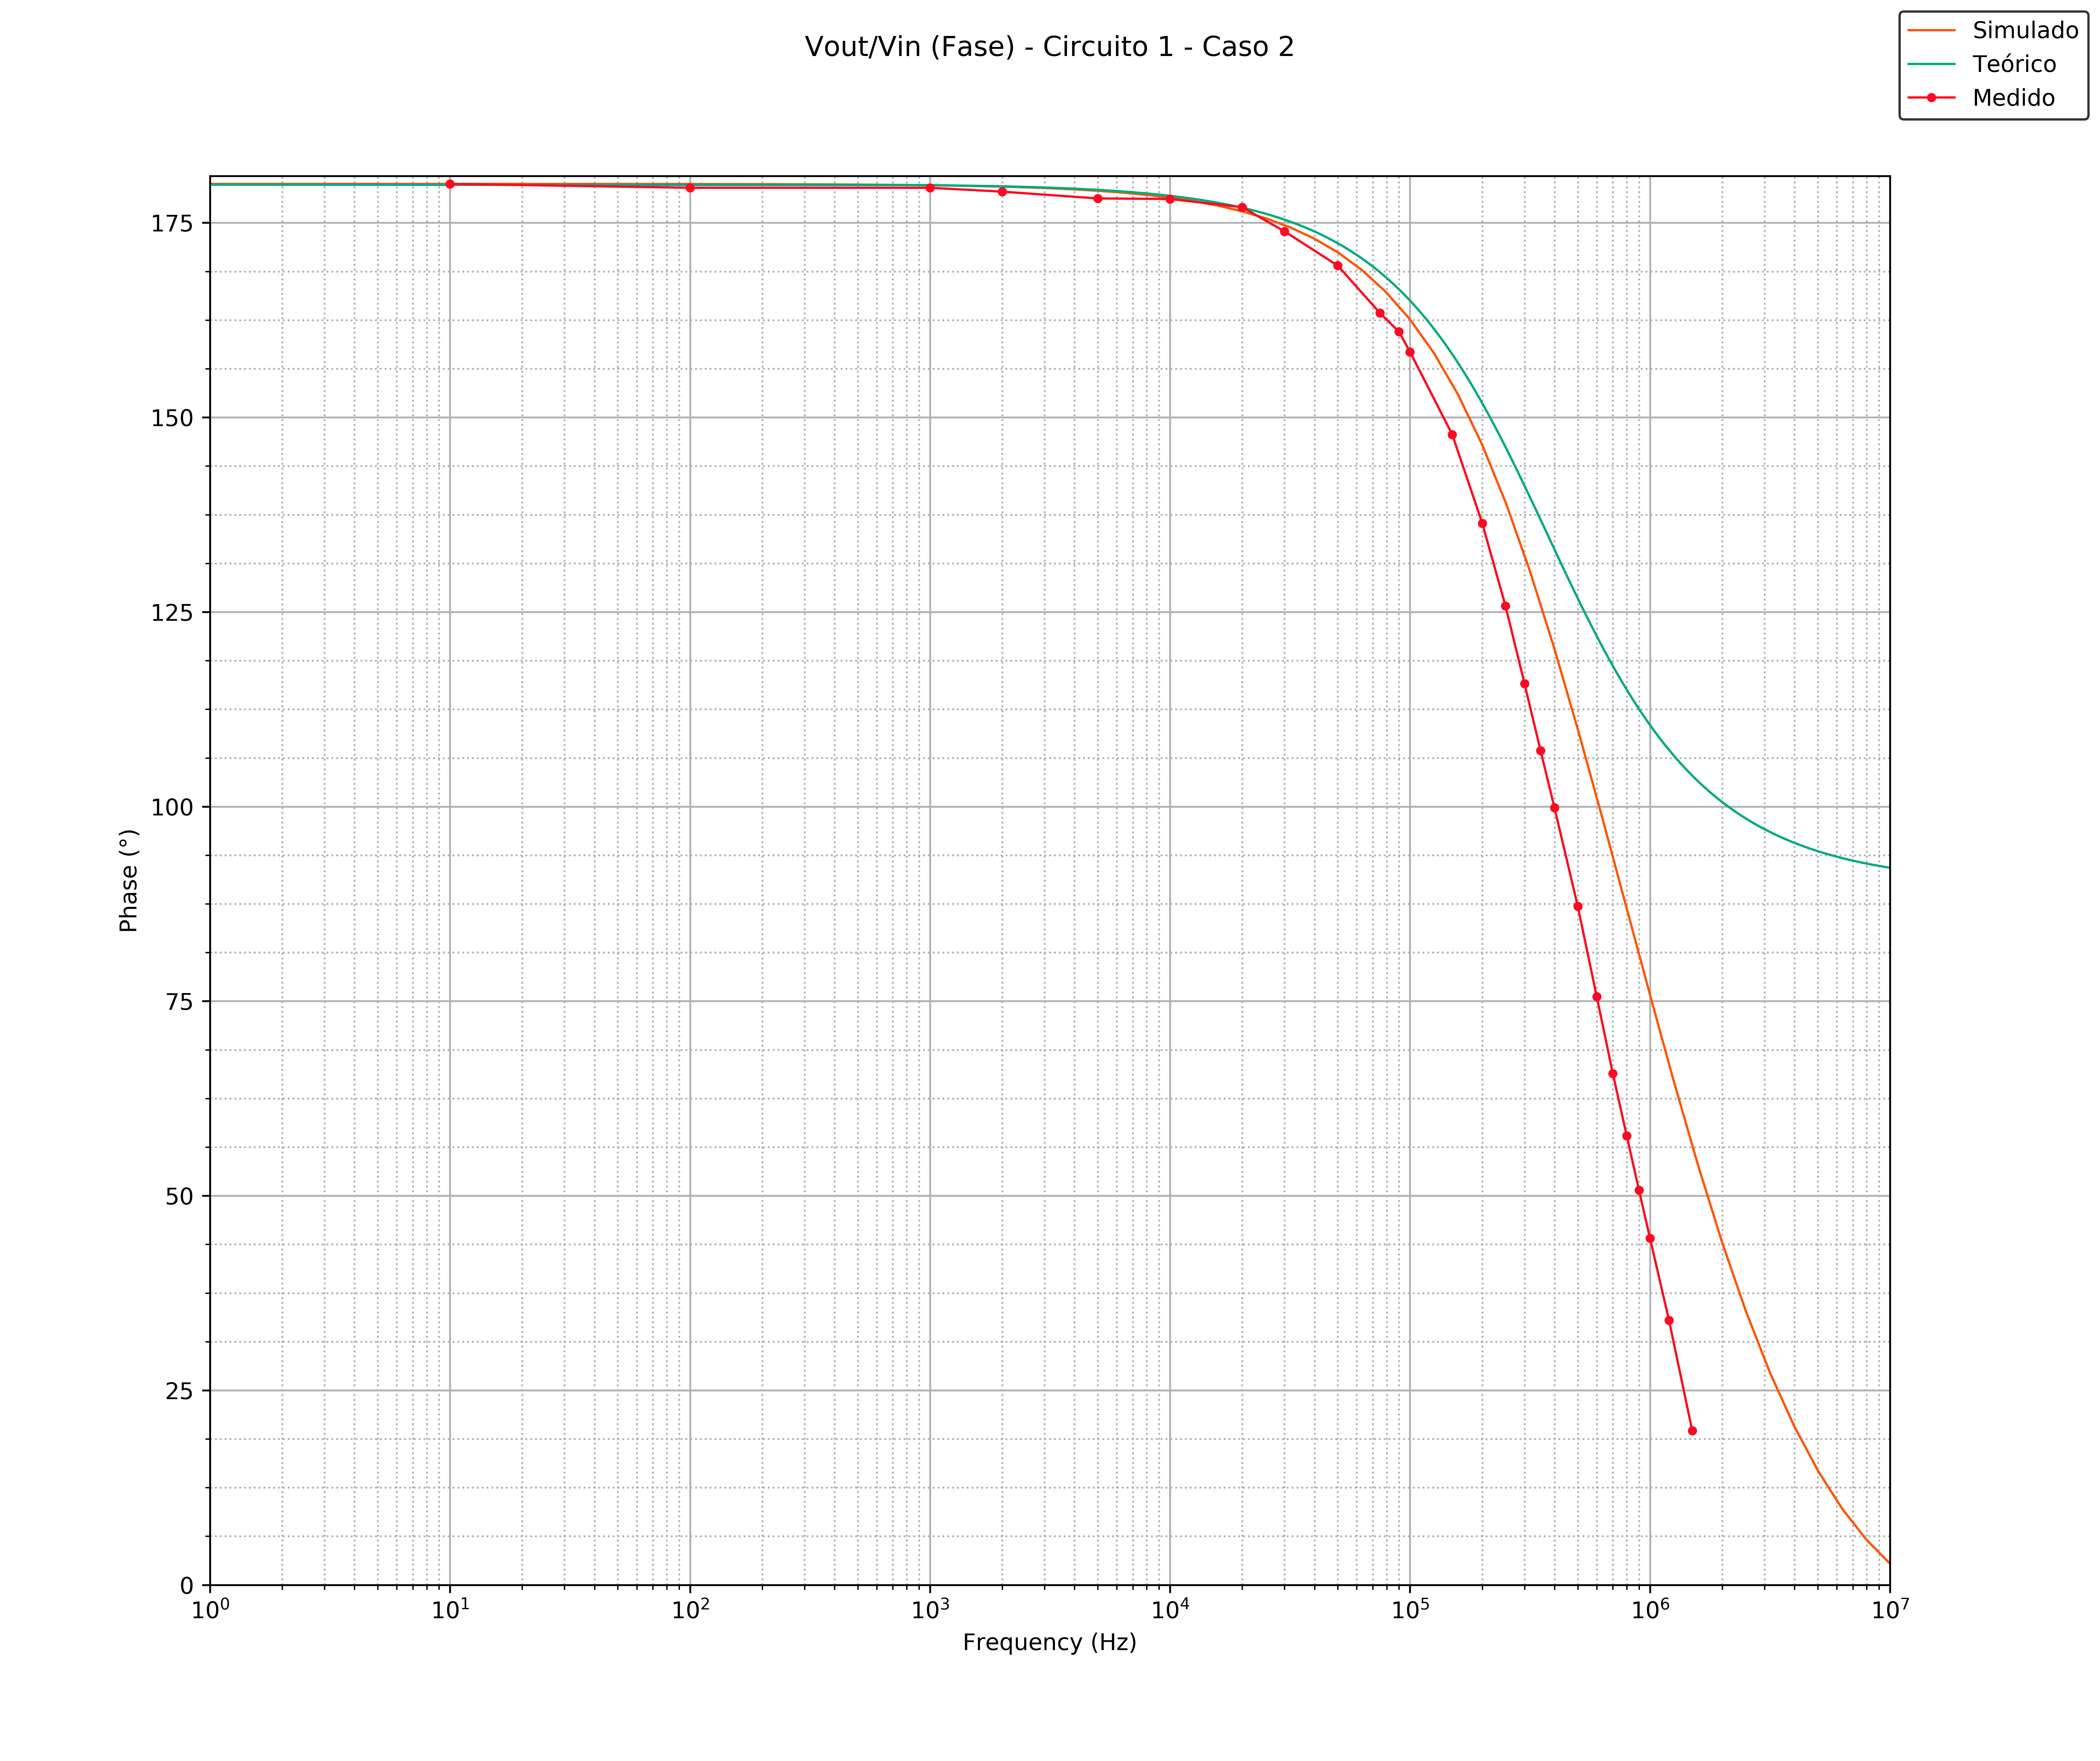
\includegraphics[width=10cm,height=10cm,keepaspectratio]{../EJ1/00GRAFICOS/c1c2/c1c2voviFASE.png}
	\caption{Configuración inversora - Caso 2 - Fase de $V_{out}/V_{in}$ }
	\label{c1c2voviP}
\end{figure}

\begin{figure}[H] %!ht
	\centering
	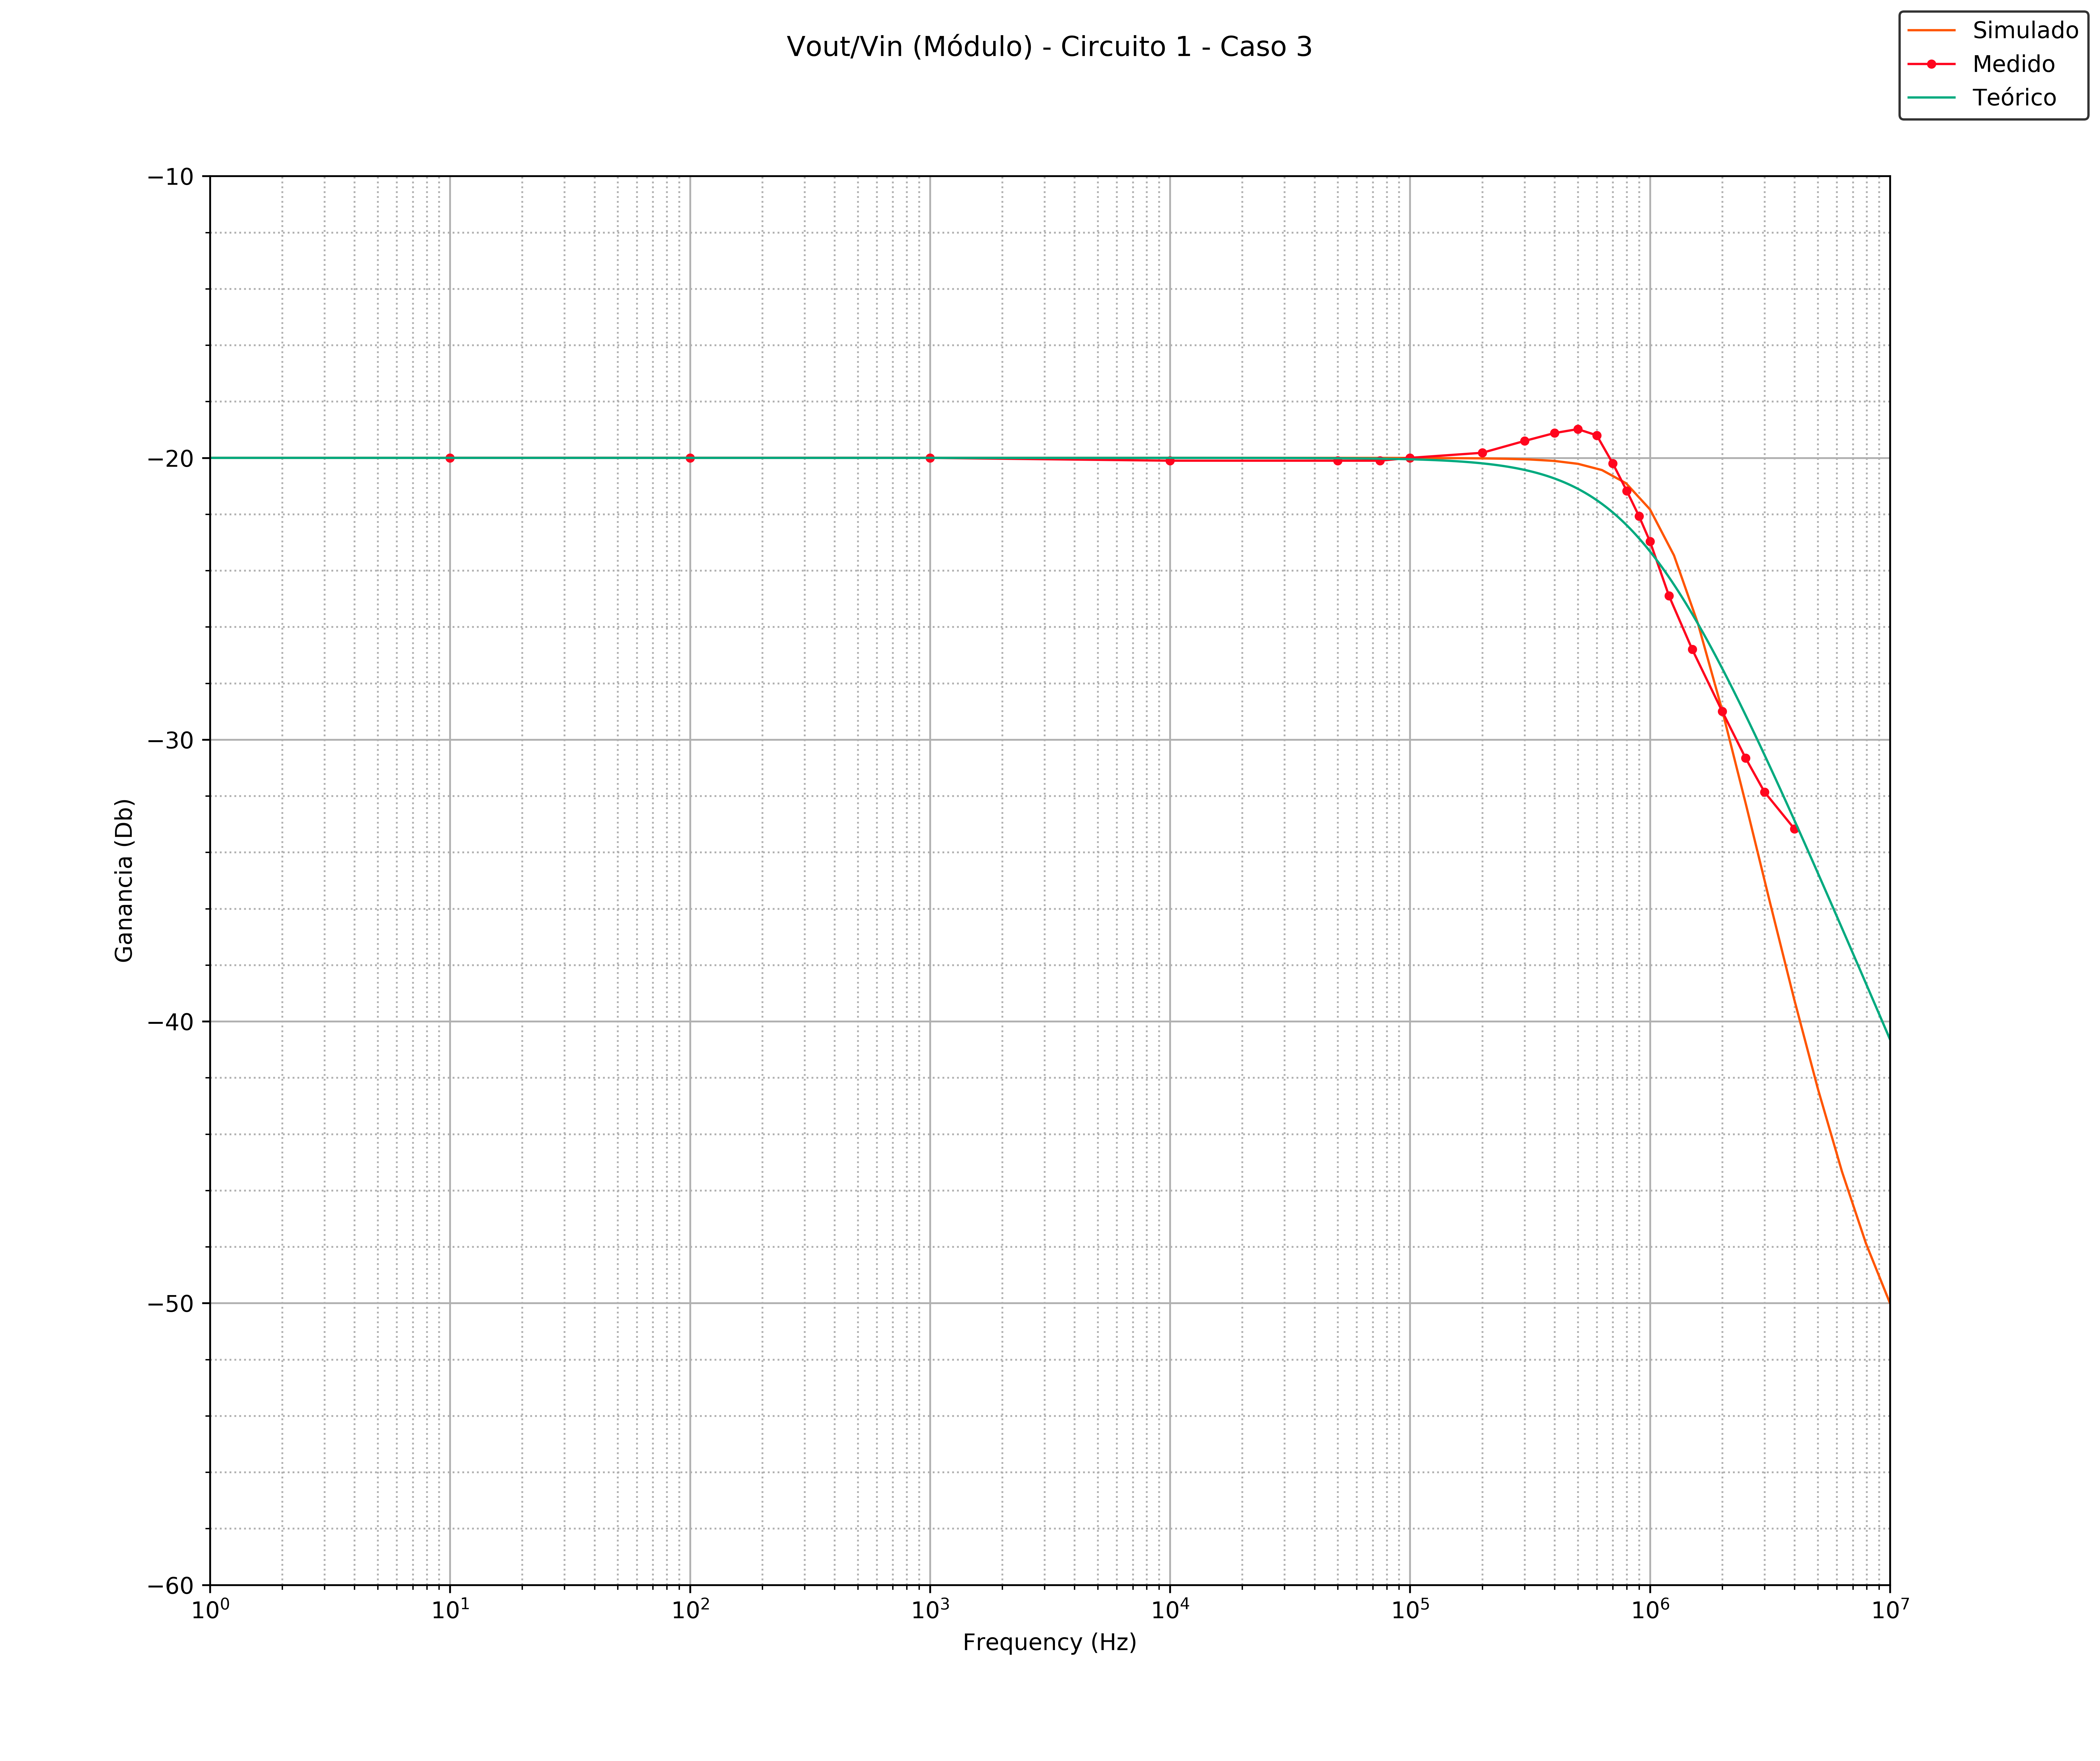
\includegraphics[width=10cm,height=10cm,keepaspectratio]{../EJ1/00GRAFICOS/c1c3/c1c3voviMod.png}
	\caption{Configuración inversora - Caso 3 - M\'odulo de$V_{out}/V_{in}$}	
	\label{c1c3voviM}
\end{figure}

\begin{figure}[H] %!ht
	\centering
	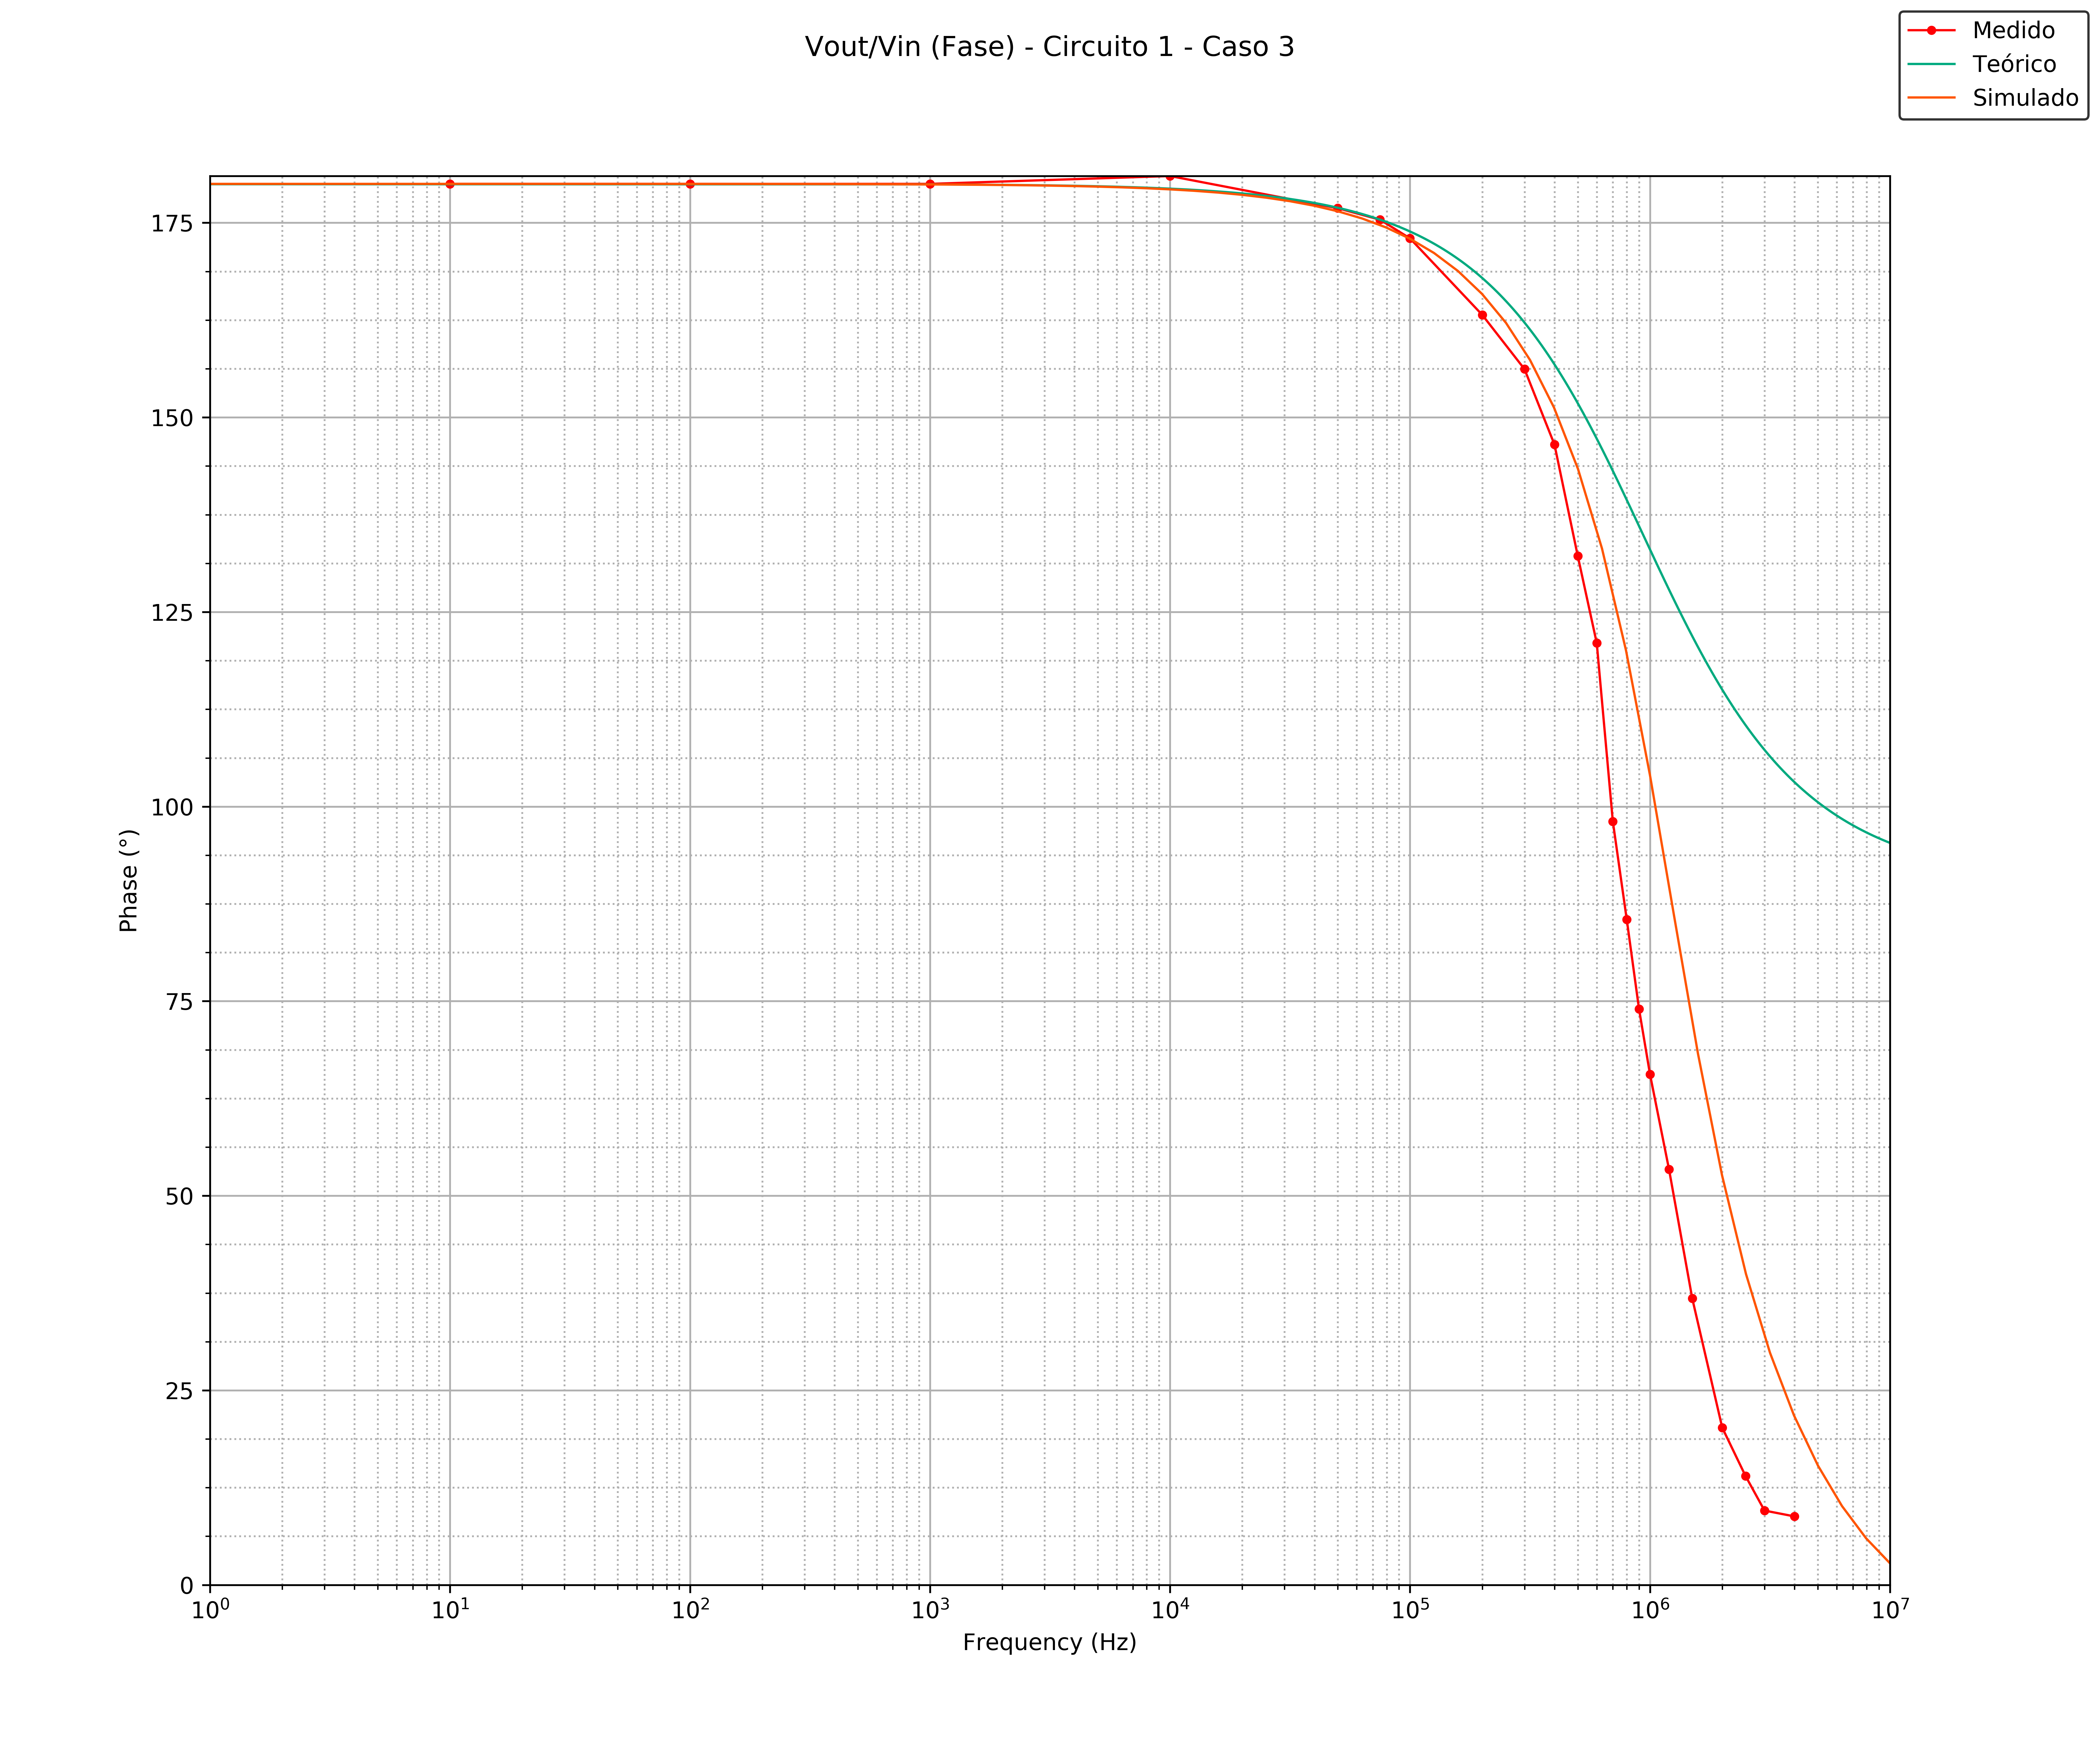
\includegraphics[width=10cm,height=10cm,keepaspectratio]{../EJ1/00GRAFICOS/c1c3/c1c3voviFASE.png}
	\caption{Configuración inversora - Fase de $V_{out}/V_{in}$}
	\label{c1c3voviP}
\end{figure}

\subsubsection*{Configuraci\'on no inversora}

\begin{figure}[H] %!ht
	\centering
	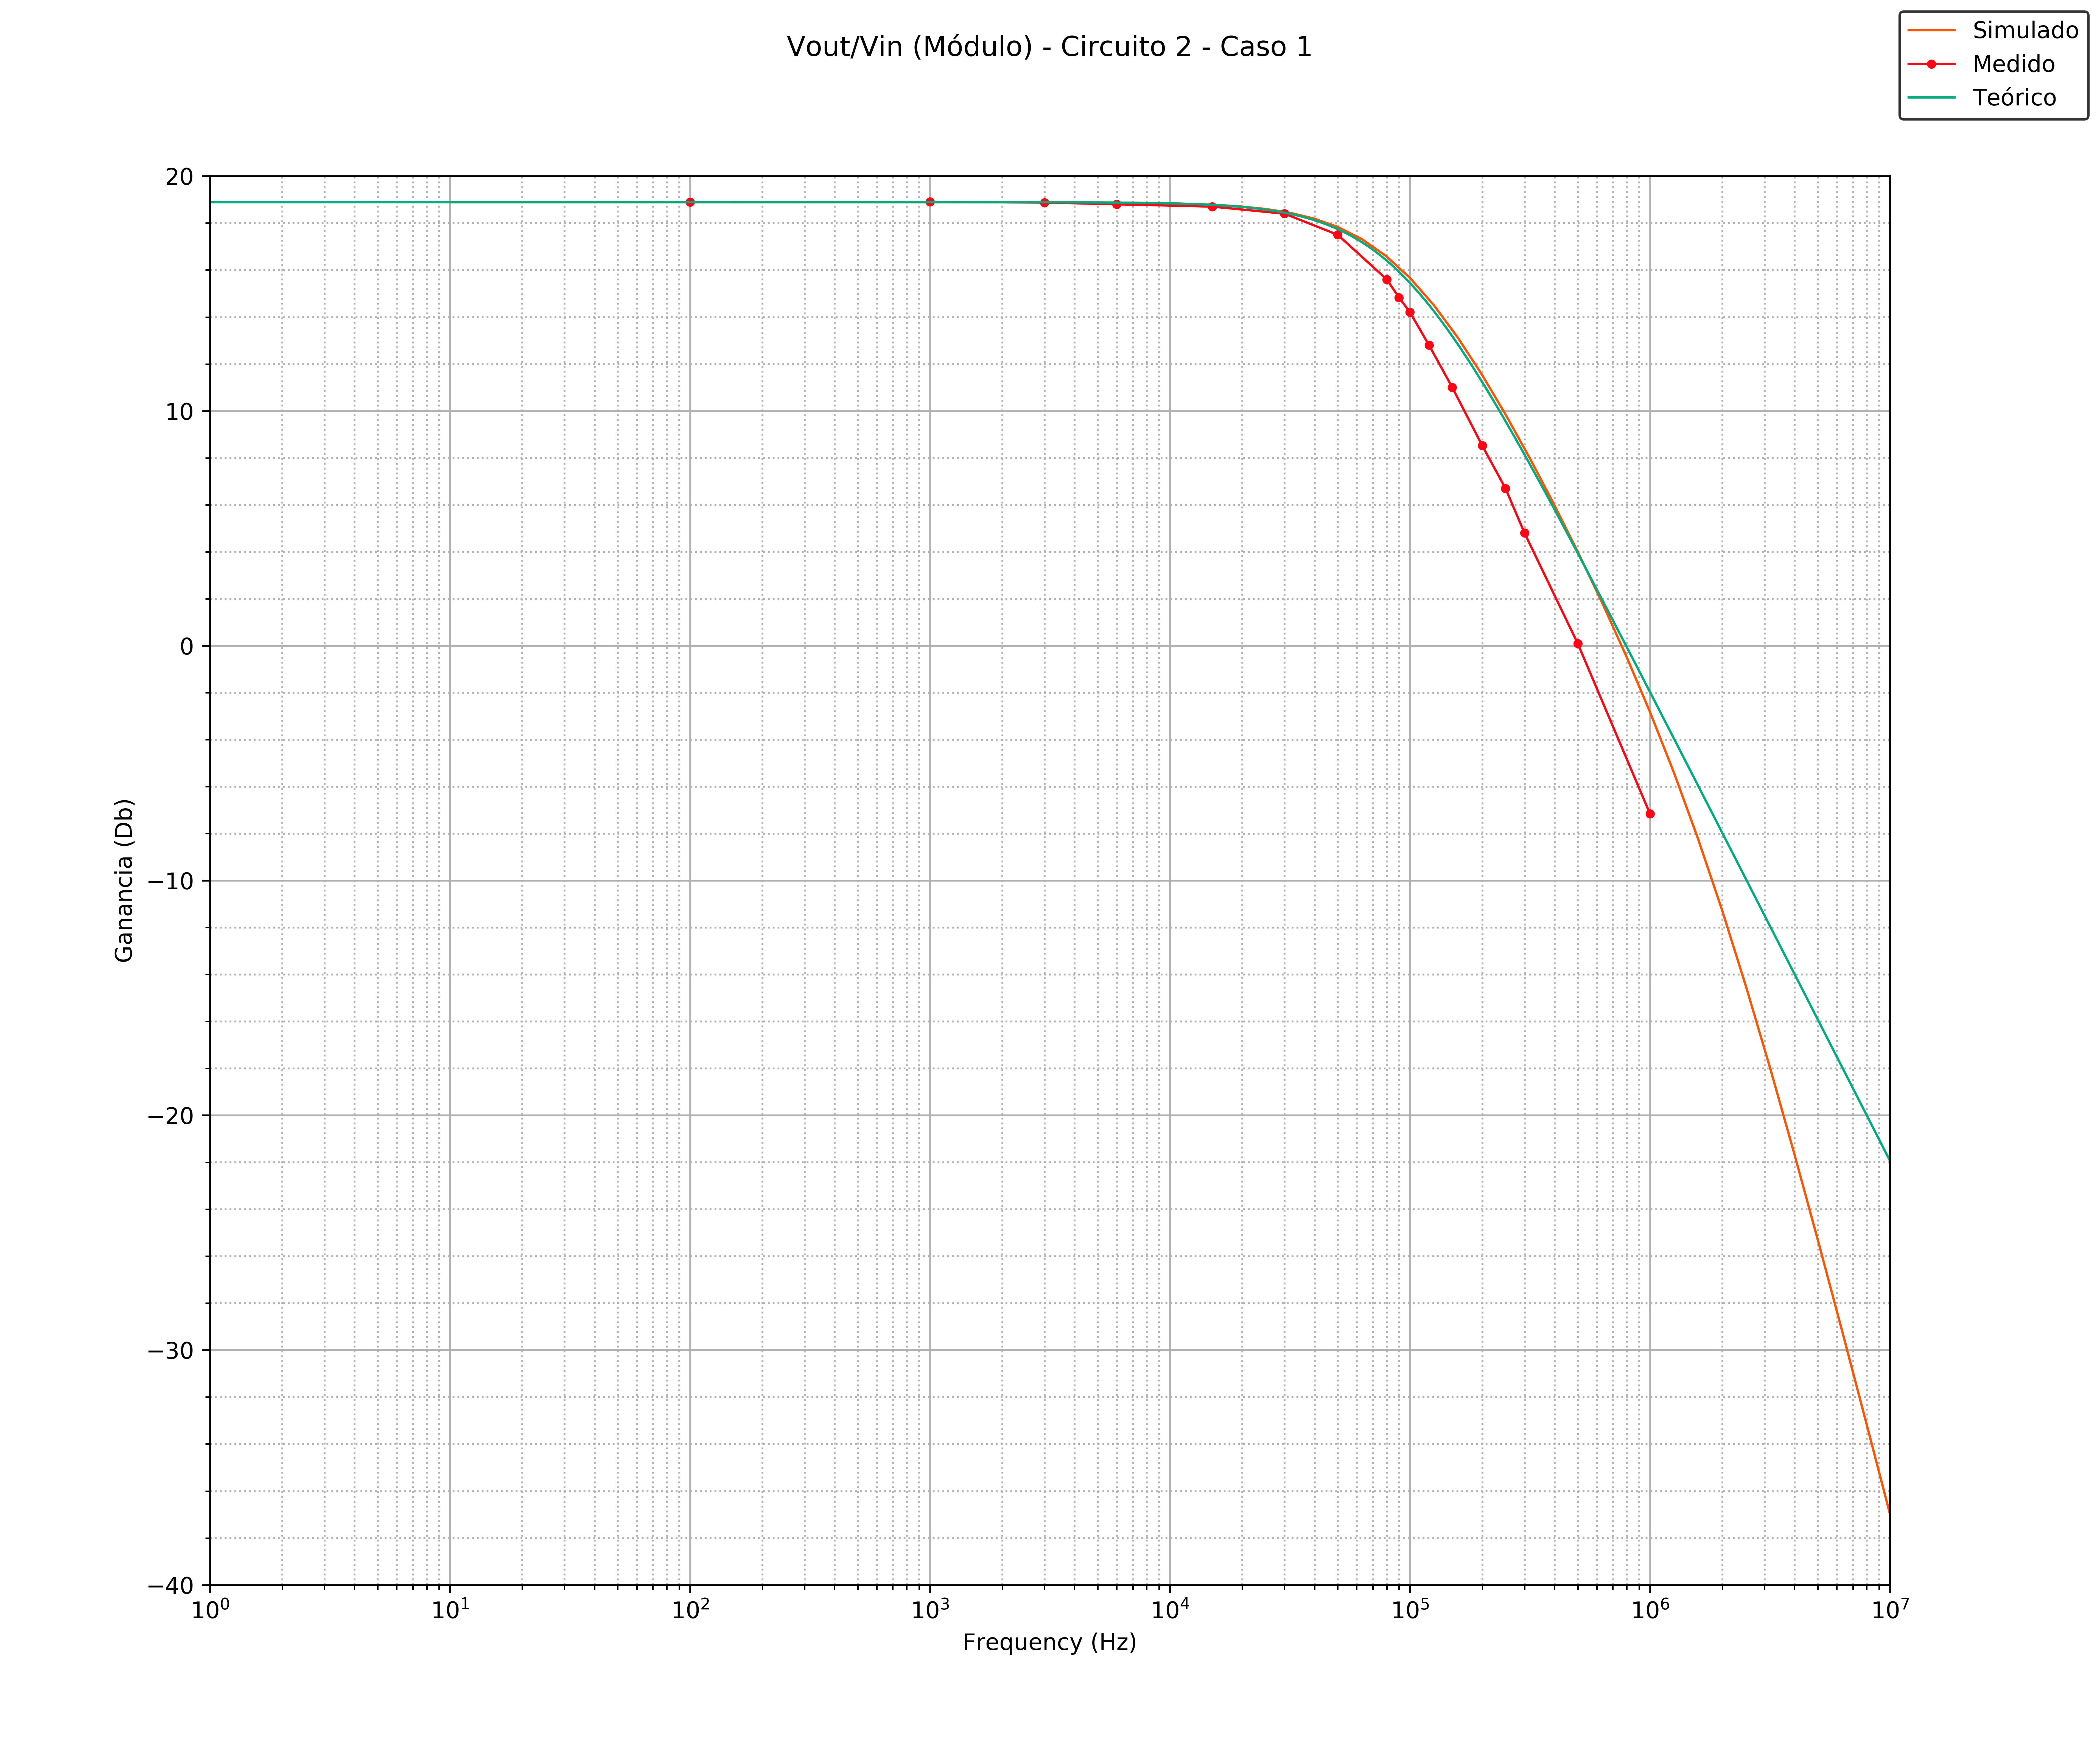
\includegraphics[width=10cm,height=10cm,keepaspectratio]{../EJ1/00GRAFICOS/c2c1/c2c1voviMod.png}
	\caption{Configuración no inversora - Caso 1 -  M\'odulo de $V_{out}/V_{in}$}
	\label{c2c1voviM}
\end{figure}

\begin{figure}[H] %!ht
	\centering
	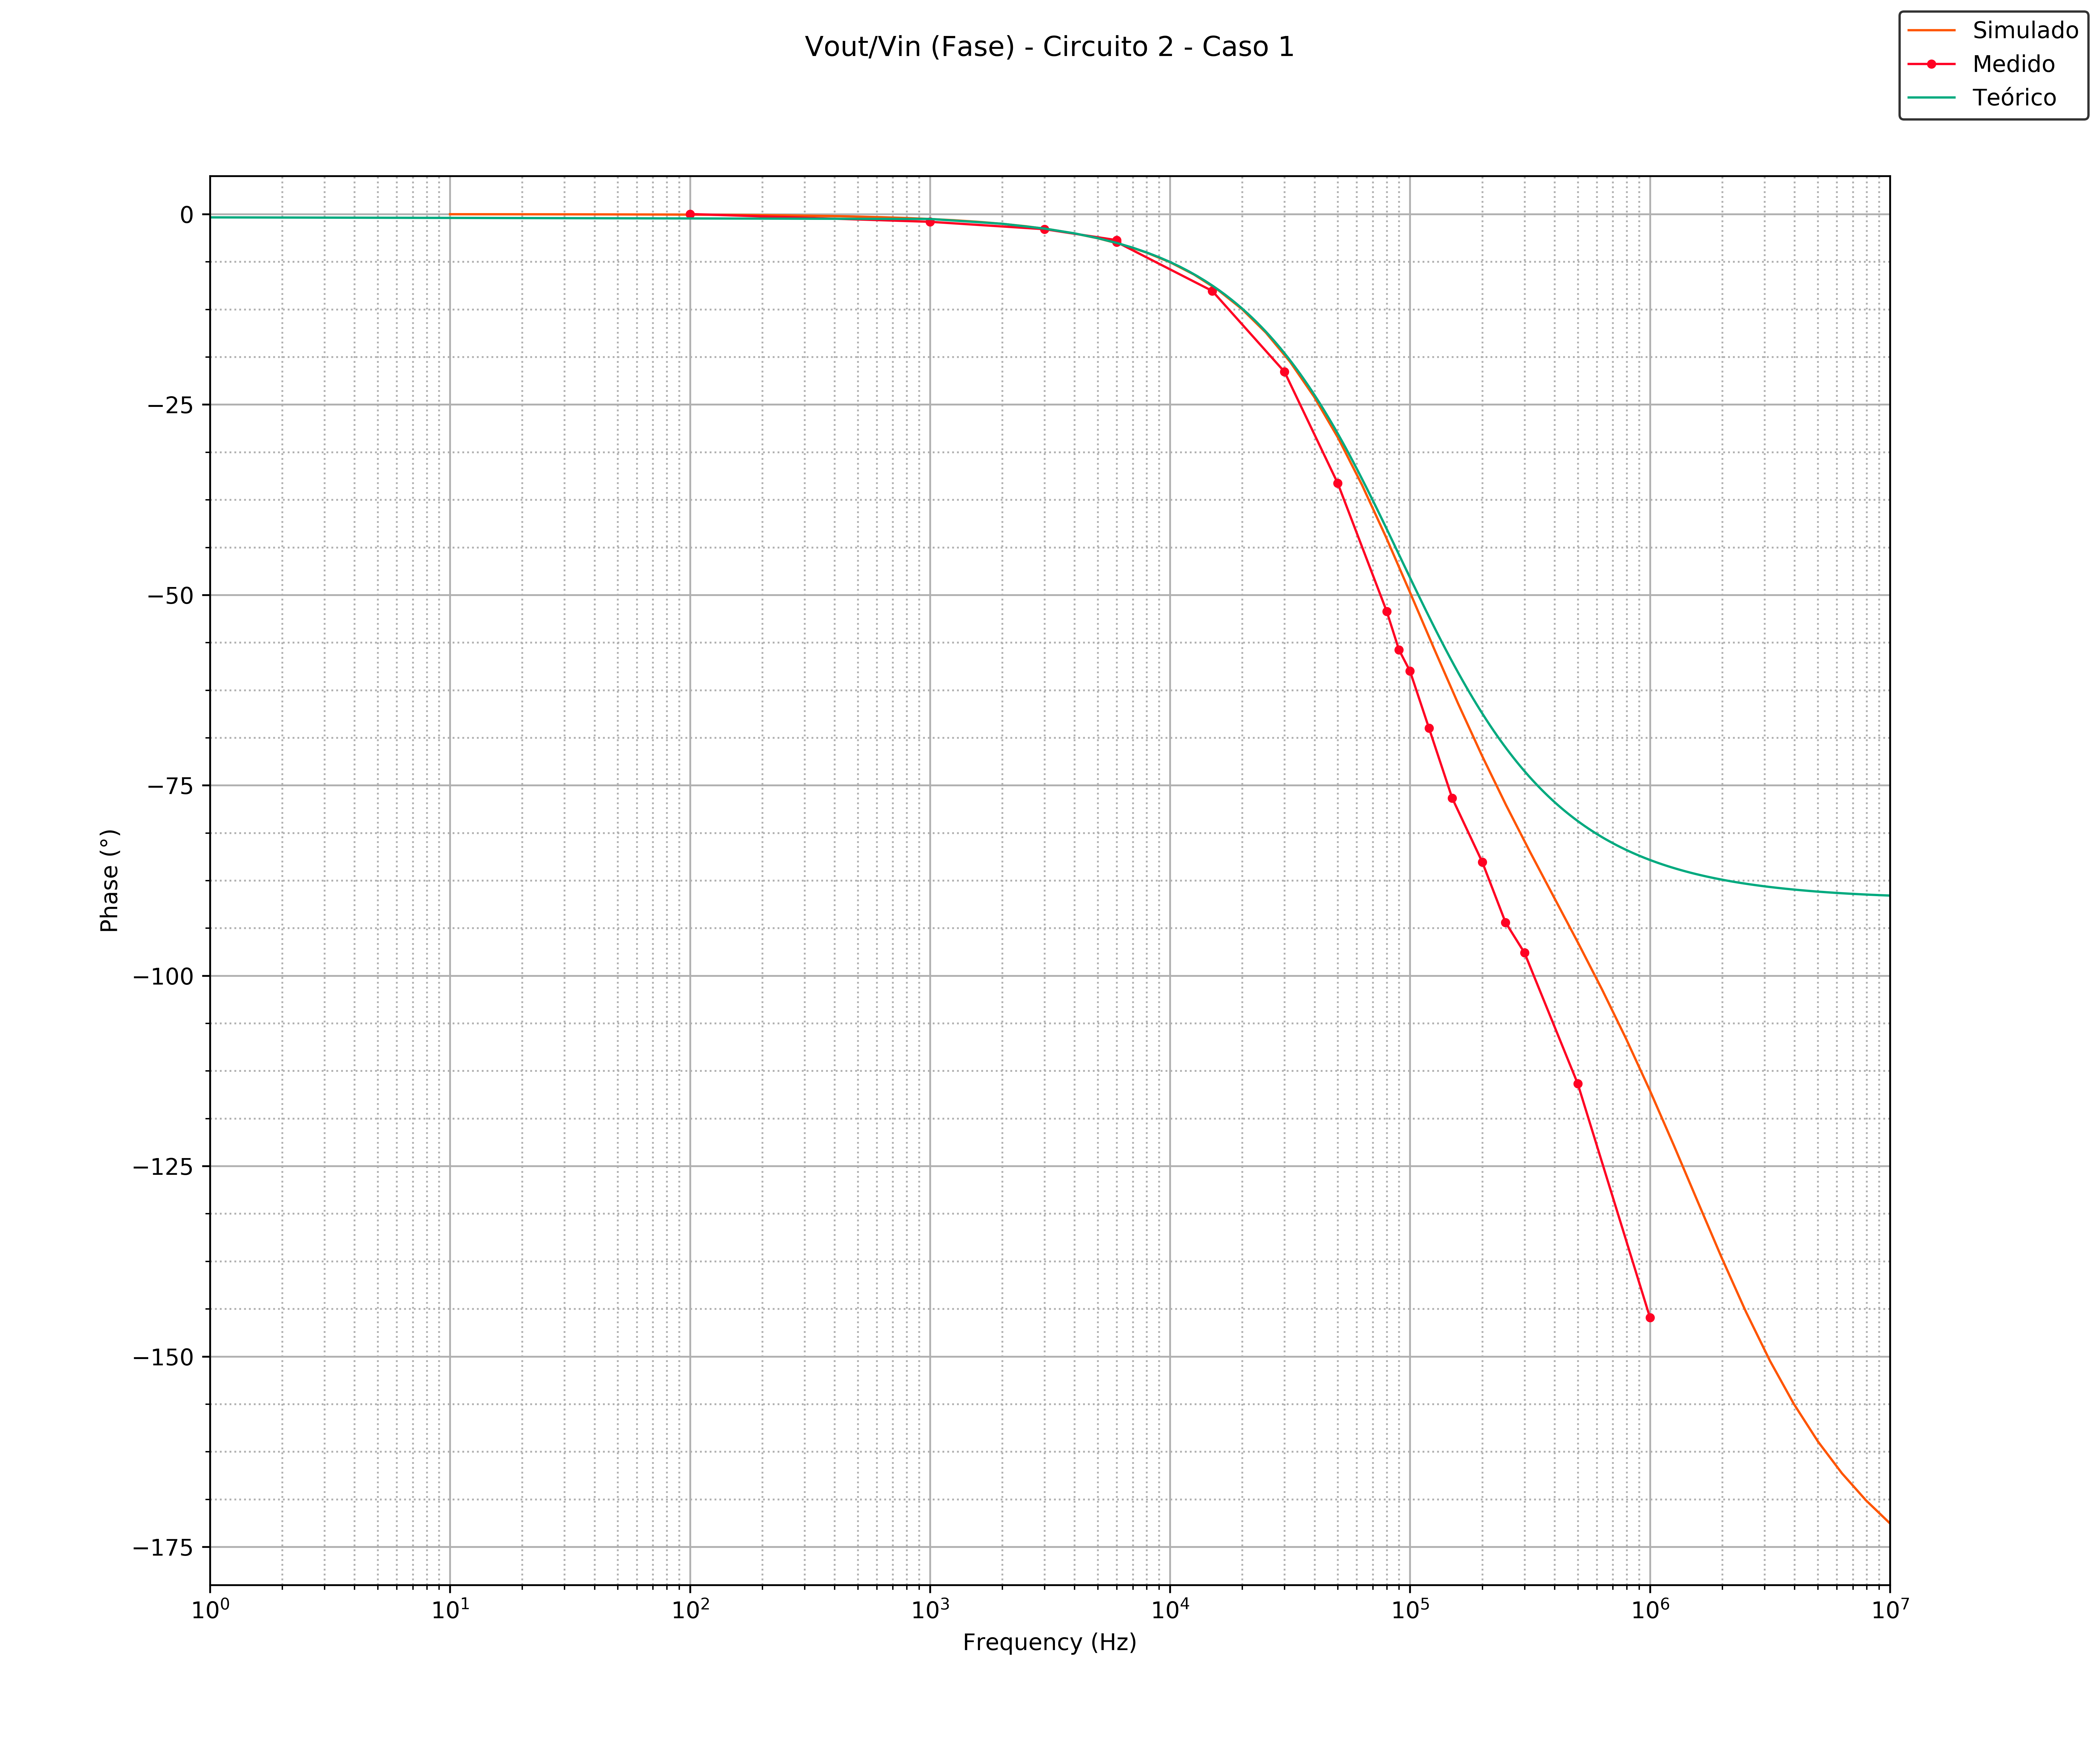
\includegraphics[width=10cm,height=10cm,keepaspectratio]{../EJ1/00GRAFICOS/c2c1/c2c1voviFASE.png}
	\caption{Configuración no inversora - Caso 1 - Fase de $V_{out}/V_{in}$}
	\label{c2c1voviP}
\end{figure}

\begin{figure}[H] %!ht
	\centering
	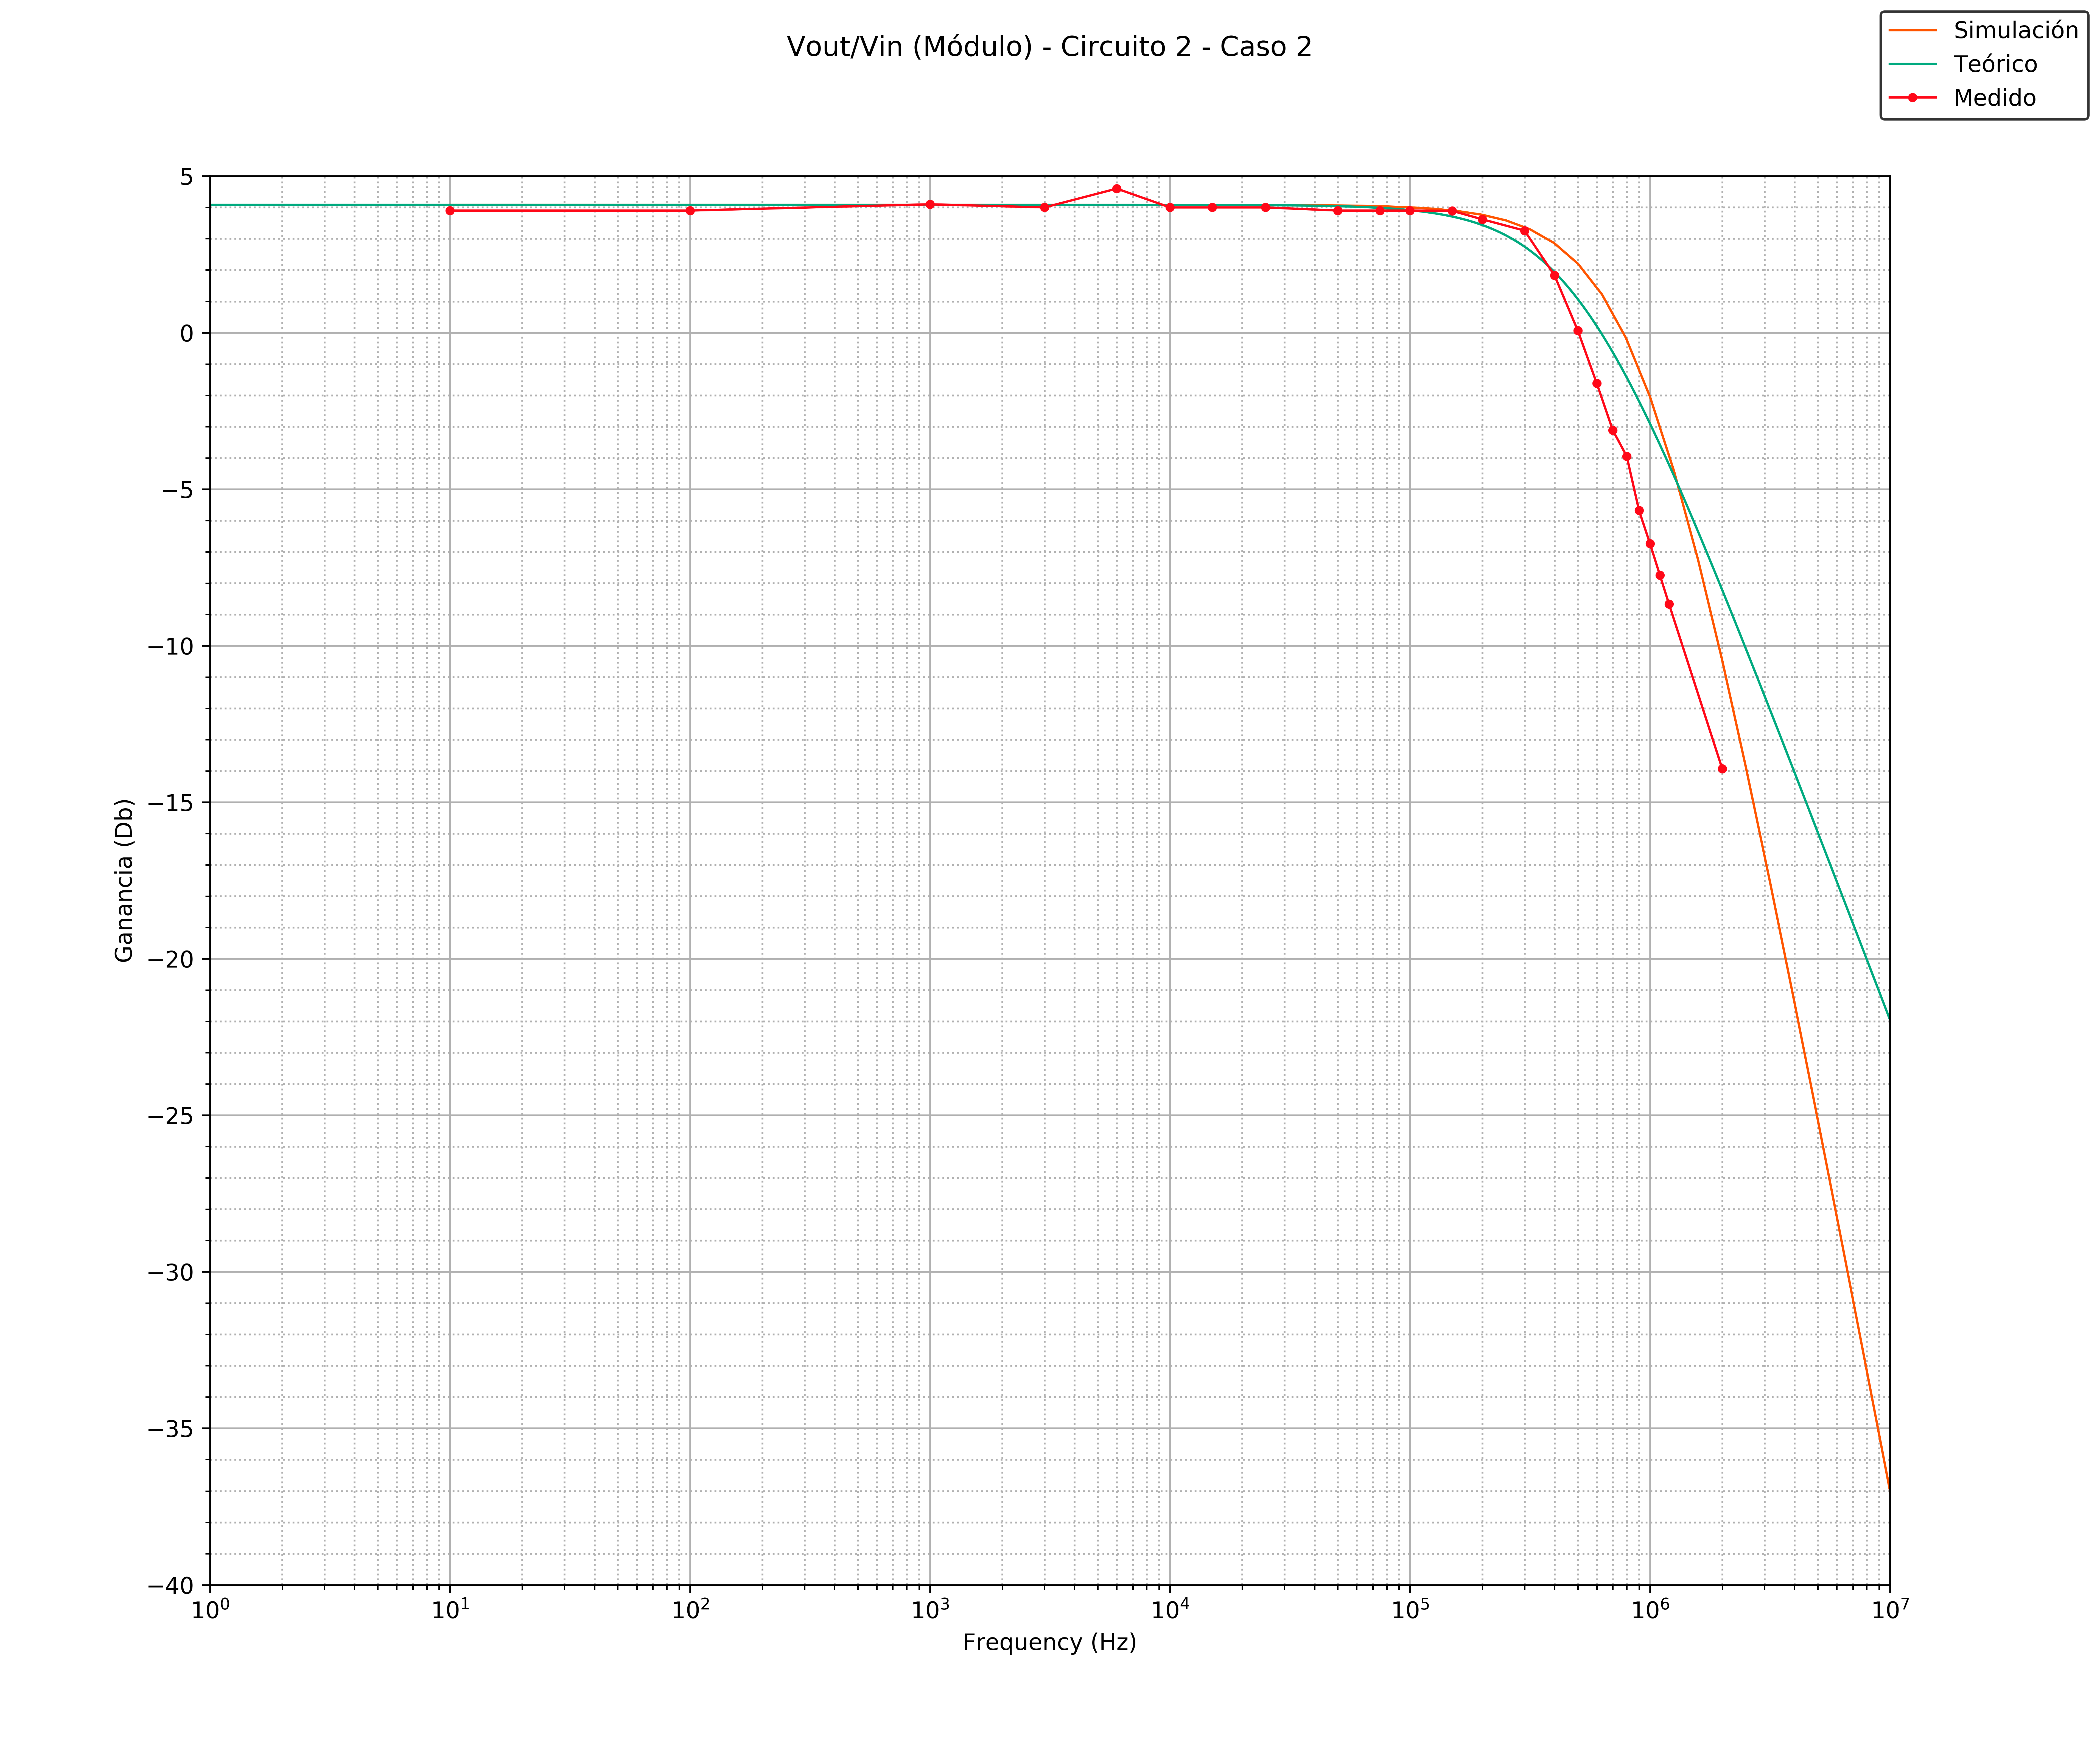
\includegraphics[width=10cm,height=10cm,keepaspectratio]{../EJ1/00GRAFICOS/c2c2/c2c2voviMod.png}
	\caption{Configuración no inversora - Caso 2 - M\'odulo de $V_{out}/V_{in}$}
	\label{c2c2voviM}
\end{figure}

\begin{figure}[H] %!ht
	\centering
	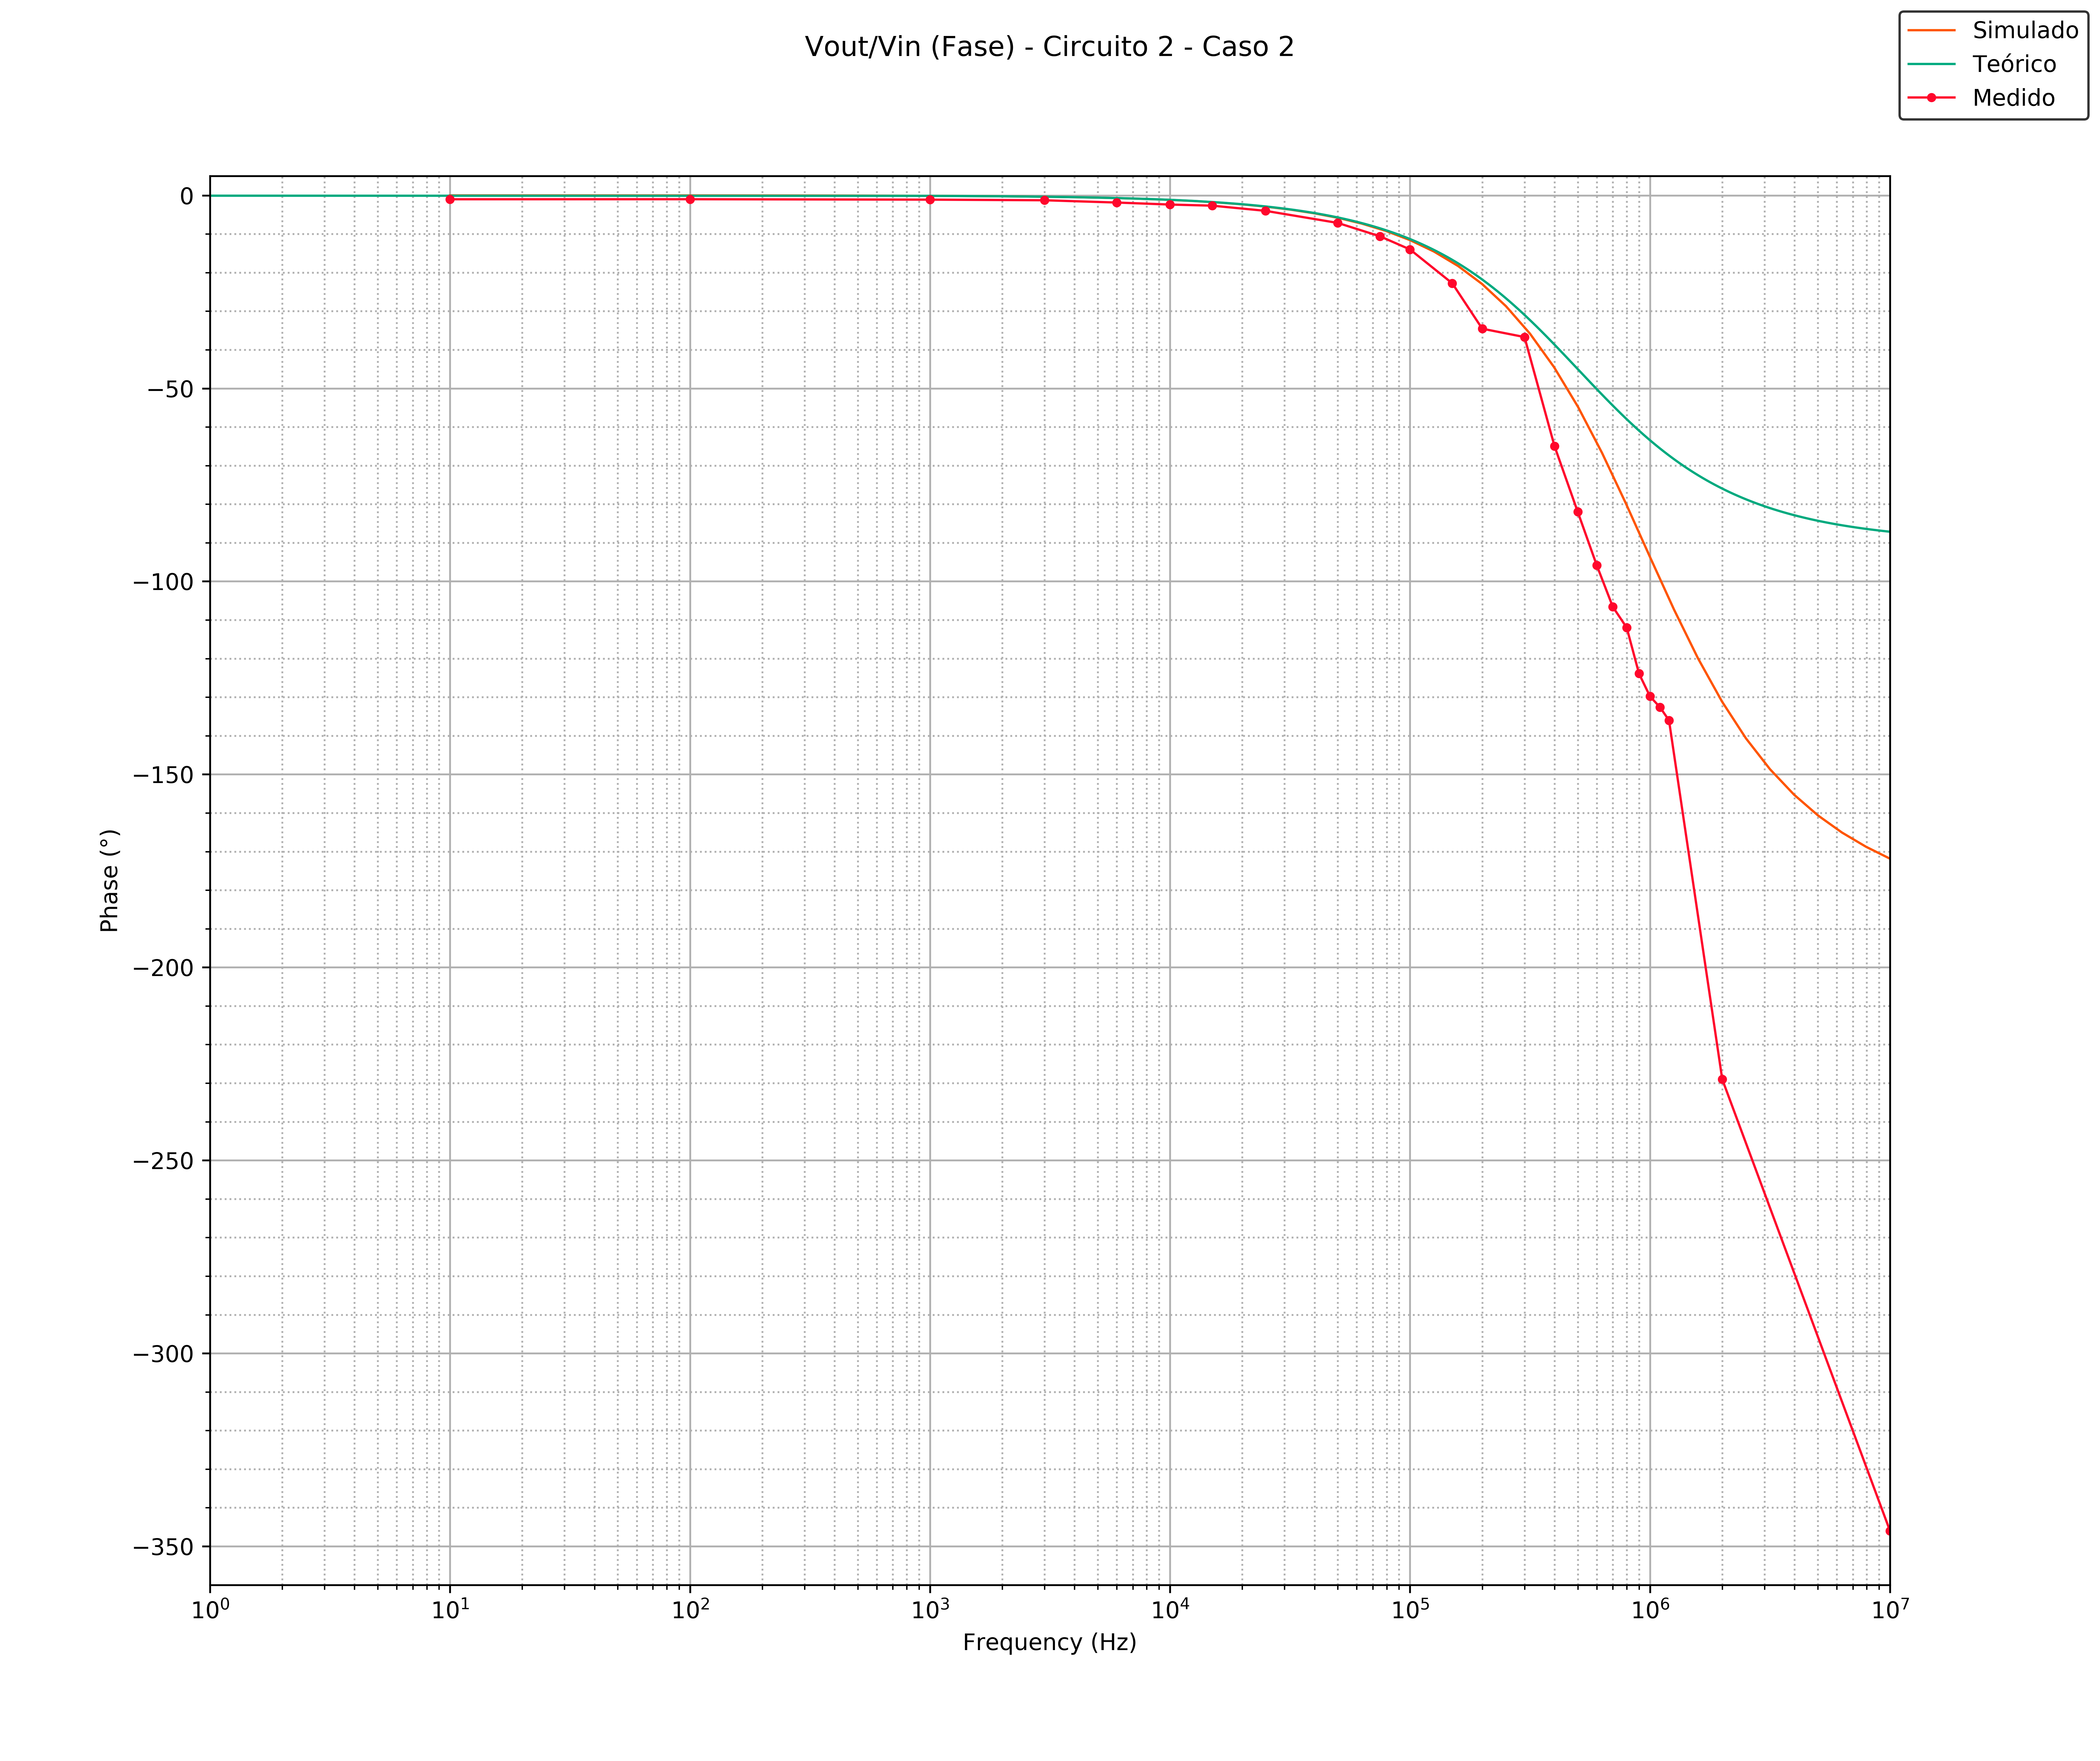
\includegraphics[width=10cm,height=10cm,keepaspectratio]{../EJ1/00GRAFICOS/c2c2/c2c2voviFASE.png}
	\caption{Configuración no inversora - Caso 2 - Fase de $V_{out}/V_{in}$}
	\label{c2c2voviP}
\end{figure}

%\begin{figure}[H] %!ht
%	\centering
%	\includegraphics[width=10cm,height=10cm,keepaspectratio]{../EJ1/00GRAFICOS/c2c3/c2c3voviMod.png}
%	\caption{Configuración no inversora - Caso 3 - M\'odulo de $V_{out}/V_{in}$}	
%	\label{c2c3voviM}
%\end{figure}

\begin{figure}[H] %!ht
	\centering
	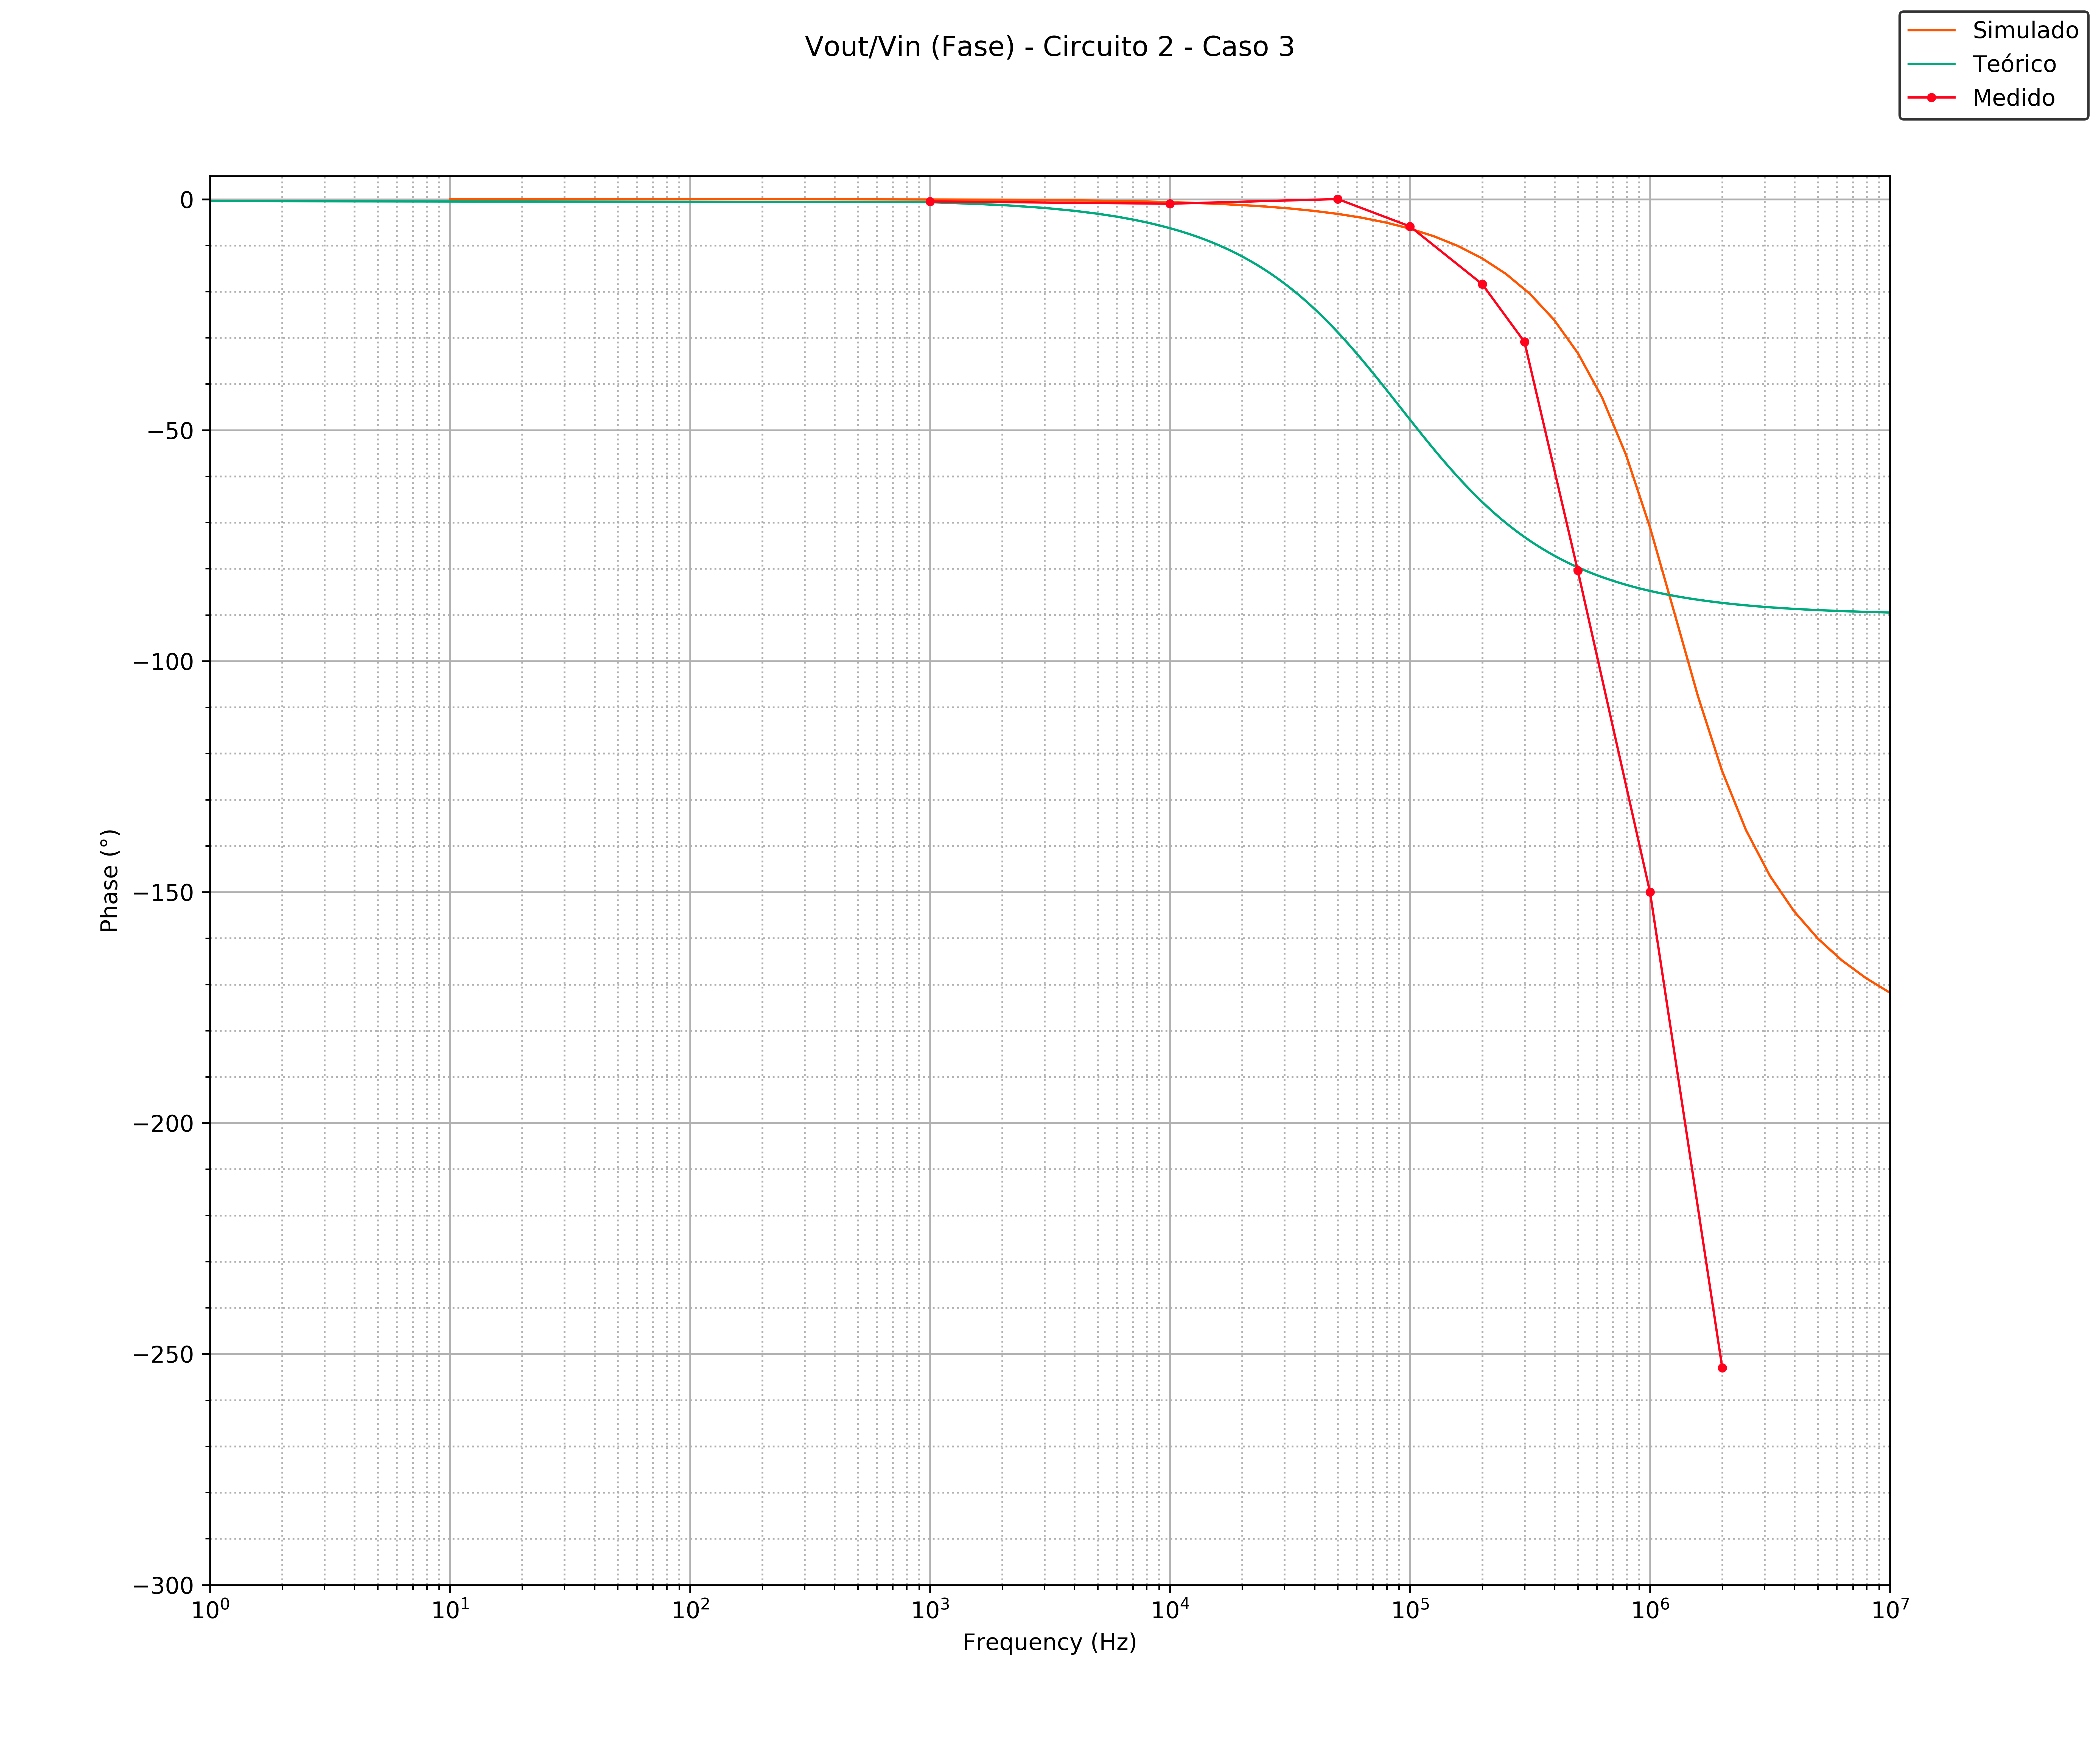
\includegraphics[width=10cm,height=10cm,keepaspectratio]{../EJ1/00GRAFICOS/c2c3/c2c3voviFASE.png}
	\caption{Configuración no inversora - Caso 3 - Fase de $V_{out}/V_{in}$}
	\label{c2c3voviP}
\end{figure}



